\ifdefined\isphone
  \documentclass[a6paper,11pt,oneside]{book}

\usepackage{algpseudocode}
\usepackage{algorithm}
\usepackage{amsfonts}
\usepackage{amsmath,amsthm,amssymb}
\usepackage{graphicx}
\usepackage{hyperref}
\usepackage{mathtools}
\usepackage{steinmetz}
\usepackage{fancyvrb}
\usepackage{textcomp}
\usepackage{gensymb}
\usepackage[normalem]{ulem}
\usepackage[T1]{fontenc}
\usepackage{cmap}
\usepackage{xspace}

\DeclareGraphicsExtensions{.pdf,.png,.jpg}

\newcommand{\mb}[1]{\ensuremath{\mathbb{{#1}}}}
\newcommand{\setof}[1]{\ensuremath{\left \{ #1 \right \}}}
\newcommand{\tuple}[1]{\ensuremath{\left \langle #1 \right \rangle }}

\DeclarePairedDelimiter{\ceil}{\lceil}{\rceil}
\DeclarePairedDelimiter{\floor}{\lfloor}{\rfloor}

\DeclareSymbolFont{bbold}{U}{bbold}{m}{n}
\DeclareSymbolFontAlphabet{\mathbbold}{bbold}

\newtheorem{statement}{Statement}
\newtheorem{rmk}{Remark}
\newtheorem{defi}{Definition}
\newtheorem{example}{Example}
\newtheorem{theorem}{Theorem}
\newtheorem{lemma}[theorem]{Lemma}
\newtheorem{proposition}[theorem]{Proposition}
\newtheorem{pf}[theorem]{Proof}
\newtheorem{corollary}[theorem]{Corollary}

% Differences
\usepackage[margin=5mm]{geometry}
\usepackage{tgheros}
\renewcommand*\familydefault{\sfdefault}

\else
  \documentclass[11pt,oneside]{book}

\usepackage{algpseudocode}
\usepackage{algorithm}
\usepackage{amsfonts}
\usepackage{amsmath,amsthm,amssymb}
\usepackage{graphicx}
\usepackage{hyperref}
\usepackage{mathtools}
\usepackage{steinmetz}
\usepackage{fancyvrb}
\usepackage{textcomp}
\usepackage{gensymb}
\usepackage[normalem]{ulem}
\usepackage[T1]{fontenc}
\usepackage{cmap}
\usepackage{xspace}

\DeclareGraphicsExtensions{.pdf,.png,.jpg}

\newcommand{\mb}[1]{\ensuremath{\mathbb{{#1}}}}
\newcommand{\setof}[1]{\ensuremath{\left \{ #1 \right \}}}
\newcommand{\tuple}[1]{\ensuremath{\left \langle #1 \right \rangle }}

\DeclarePairedDelimiter{\ceil}{\lceil}{\rceil}
\DeclarePairedDelimiter{\floor}{\lfloor}{\rfloor}

\DeclareSymbolFont{bbold}{U}{bbold}{m}{n}
\DeclareSymbolFontAlphabet{\mathbbold}{bbold}

\newtheorem{statement}{Statement}
\newtheorem{rmk}{Remark}
\newtheorem{defi}{Definition}
\newtheorem{example}{Example}
\newtheorem{theorem}{Theorem}
\newtheorem{lemma}[theorem]{Lemma}
\newtheorem{proposition}[theorem]{Proposition}
\newtheorem{pf}[theorem]{Proof}
\newtheorem{corollary}[theorem]{Corollary}

% Differences
\setlength{\textheight}{9.5in}
\setlength{\textwidth}{7.0in}
\setlength{\topmargin}{-0.75in}
\setlength{\oddsidemargin}{-0.25in}
\setlength{\evensidemargin}{0.75in}
\setlength{\parskip}{0.15in}
\setlength{\parindent}{0in}

\fi

\usepackage{listings}
\usepackage[usenames,dvipsnames]{color}

\newcommand{\appr}{\textsc{approx}\xspace}
\newcommand{\ptas}{\textsc{ptas}\xspace}
\newcommand{\fptas}{\textsc{fptas}\xspace}
\newcommand{\npcomplete}{\textsc{NP-complete}\xspace}
\newcommand{\np}{\textsc{NP}\xspace}
\newcommand{\nphard}{\textsc{NP-hard}\xspace}
\newcommand{\open}{\textsc{open}\xspace}
\newcommand{\opt}{\textsc{opt}\xspace}
\newcommand{\p}{\textsc{P}\xspace}

\providecommand{\myceil}[1]{\left \lceil #1 \right \rceil }
\providecommand{\myfloor}[1]{\left \lfloor #1 \right \rfloor }
\newcommand{\Thm}{\textbf{Theorem}\xspace}
\newcommand{\Prf}{\textbf{Proof}\xspace}

% TODOs:
%   Clarifications:
%       What is fractional cascading?
%       What does '2 claims means that $1.5n$ comparisons in the worst case' refer to?
%       Where did Fibonacci Heaps go? (once done, we can link to them from the place we reference them from)

% Course Name
\title{CS 466 \\
F13}

% Fill in your name.
\author{By: Shale Craig \\
Prof: Anna Lubiw \\
\\ \\ \\
Adapted From Notes In Class and External Sources}

% Set the default pseudocode language:
\lstset{language=Python} % Almost-python.

% Now we will begin writing the document.
\begin{document}
    \maketitle

    % Next, we need to make a Table of Contents, List of Figures and
    % List of Tables.  You will most likely need to run LaTeX twice to
    % get these correct.  The first pass for LaTeX to figure out the
    % labels, and the second pass to put in the right references.
    \tableofcontents

    %%%%%%%%%%%%%%%%%%%%%%%%%%%%%%%%%%%%%%%%%%%%%%%%%%%%%%%%%%%%%%%%%%%%%
    %% REPORT BODY
    %%%%%%%%%%%%%%%%%%%%%%%%%%%%%%%%%%%%%%%%%%%%%%%%%%%%%%%%%%%%%%%%%%%%%
    %% \main will make the \section commands numbered again,
    %% it will also use arabic page numbers.
    \mainmatter

    \chapter{Introduction} % (fold)
    \label{cha:introduction}
        In this course, we want to solve algorithmic problems, and compounding general knowledge with developments of the last 30 years.
        Though these notes are grouped by lecture, this course can be split into three sections:
        \begin{enumerate}
            \item Algorithmic Design
            \begin{itemize}
                \item Assumed knowledge of greedy, divide \& conquer, and dynamic programming techniques
                \item Introduction to randomization, approximation, and online algorithmic techniques
            \end{itemize}
            \item Algorithmic Analysis
            \begin{itemize}
                \item Assumed knowledge of big $O$, worst case asymptotic analysis techniques
                \item Introduction to amortized analysis, probabilistic analysis, and approximation factors methods
            \end{itemize}
            \item Lower Bounds
            \begin{itemize}
                \item Understanding of \npcomplete-ness is assumed
                \item Hardness of approximation is introduced
            \end{itemize}
        \end{enumerate}
        The class website is \url{https://www.student.cs.uwaterloo.ca/~cs466/}.

        \section{TSP} % (fold)
        \label{sec:tsp}
            \subsection{Problem Statement} % (fold)
            \label{sub:problem_statement}
                % TODO: I messed up on the footnotes here. Make them agree again.
                Given a graph $G = (V, E)$ with weights on edges $w : E \to R$, find a \uline{TSP tour}\footnote{A tour is a traversal ordering of vertexes in a graph}, which is a Hamiltonian Tour\footnote{A Eulerian Tour is a tour that goes through each vertex exactly once and returns to the first vertex.} $C$ that visits each vertex exactly once and has minimum weight:
                \[ \sum_{e \in C} w(e) \]

                Since we can add infinite-weight edges to any non-complete graph, we assume that we have a complete graph\footnote{A complete graph is one where there exists an edge between all vertexes in the graph.}.

                \textsc{TSP} is a known \npcomplete problem.
            % subsection problem_statement (end)
            \subsection{\npcomplete} % (fold)
            \label{sub:npcomplete}
                To show a problem $R$ is \npcomplete, we need to show that both:
                \begin{enumerate}
                    \item Prove $R$ is in \np.
                    \item Give a reduction (denoted ``$\le_p$'') from a known \npcomplete problem to an instance of the $R$ problem.
                \end{enumerate}
                Thus to prove that \textsc{TSP} is \npcomplete, we need to show both:
                \begin{itemize}
                    \item \textsc{TSP} is in \np
                    \item Hamiltonian Cycle $\le_p$ \textsc{TSP}.
                \end{itemize}
                Assuming that Hamiltonian Cycle in our reduction is a known \npcomplete problem, we now know that \textsc{TSP} is \npcomplete too.

                Unless $\p = \np$, we need to choose two of these three options:
                \begin{itemize}
                    \item A \textit{speedy} algorithm
                    \item Solve the \textit{problem precisely}
                    \item Solve a \textit{hard problem}
                \end{itemize}
                \npcomplete problems are hard, so we must choose between \emph{precision} and \emph{speed} when solving them.
            % subsection npcomplete (end)
            \section{Metric \textsc{TSP}} % (fold)
            \label{sec:metric_tsp}
                We define Metric \textsc{TSP} as a weaker variant of \textsc{TSP} where the distance between two vertexes is the same in either order, and distances always follows the triangle inequality.
                \begin{align*}
                    d(u, v) &=   d(v, u) \\
                    d(u, v) &\le d(u, \beta) + d(\beta, v)
                \end{align*}

                There exists a fast approximation algorithm that exists for this problem:
                \begin{itemize}
                    \item Find minimum-spanning tree (see Chapter~\ref{cha:minimum_spanning_trees} for more information) of the graph using \href{https://en.wikipedia.org/wiki/Kruskal's_algorithm}{Kruskal's Algorithm} ($O(m \log n)$).
                    \item Take a tour walking around the tree, taking shortcuts to avoid re-visiting vertexes
                    \item The distance added by the shortcuts is less than or equal to twice the distance of remaining in the tree.
                \end{itemize}

                Here's a quick proof to this lemma:
                In a given graph, call $\ell$ the length of the tour of our algorithm, and call $\ell_{TSP}$ the distance traveled in the minimal \textsc{TSP} tour.

                We want to prove that $\ell \le 2 \ell_{TSP}$, so that this is a $2$-approximation (For more information, see Chapter~\ref{cha:approximation_algorithms}).

                We know that $\ell \le 2 \ell_{MST} \le 2 \ell_{TSP}$ since deleting one edge of a minimum \textsc{TSP} tour gives us a spanning tree.

                \textbf{Sidenote:} There exists a $1.5$ approximation, but there were no specifics given in class.
                The apparently, the idea is to use a matching algorithm.

                \subsection{Implementation} % (fold)
                \label{sub:implementation}
                    \begin{itemize}
                        \item We must find a minimum spanning tree, which takes $O(m\log n)$ time using Prim and Kruskal's Algorithm.
                            \begin{description}
                                \item[$m$] is the number of edges.
                                \item[$n$] is the number of vertexes.
                            \end{description}
                        \item We will see improved heaps in this class that allow us to take the time down to $O(m + n \log n)$
                    \end{itemize}

                    This method doesn't work for General \textsc{TSP}, since if there exists a $k$-approximation, then $\p=\np$\footnote{An approximation for this would solve the Hamiltonian-Cycle decision problem in \p time. The Hamiltonian Cycle decision problem is known to be \npcomplete.}.
                % subsection implementation (end)
            % section metric_tsp (end)
            \section{Types of \textsc{TSP}} % (fold)
            \label{sec:types_of_tsp}
                In general, the ordering is from hardest to easiest:

                General \textsc{TSP} $\ge$ Metric \textsc{TSP} $\ge$ Euclidean \textsc{TSP}

                \begin{description}
                    \item[General] is the basic ``general'' \textsc{TSP} problem.
                    \item[Metric] is described above
                    \footnote{There is a $(1.5)$-approximation algorithm, but the minimum bound is $1.0045$.}.
                    \item[Euclidean] is where vertexes are placed on a plane, and the weight of edges is the euclidean distance between vertexes
                    \footnote{There is an $(\epsilon+1)$-solution for an $\forall \epsilon > 0$, but time grows as $\epsilon$ decreases.
                    This is a \href{https://en.wikipedia.org/wiki/Polynomial-time_approximation_scheme}{Polynomial Time Approximation Scheme}. See Chapter TODO for PTASs.}.
                \end{description}
            % section types_of_tsp (end)
        % section \textsc{TSP} (end)
    % chapter introduction (end)
    \part{Data Structures} % (fold)
    \label{prt:data_ _structures_}
        Every algorithm must store, access, or search data.
        We look at amortized analysis and more complicated data structures these data structures.

        It's assumed knowledge of the following:
        \begin{itemize}
            \item Heap-based priority queue
            \item Dictionaries built using hashing, and balanced binary search.
        \end{itemize}
        \chapter{Binomial Heaps} % (fold)
        \label{cha:binomial_heaps}
            \section{Heaps} % (fold)
            \label{sec:heaps}
                Heaps store are binary trees of elements, each with an numeric key.
                For a minimum heap, the minimum key is the root.
                Usually, we shape our heap as a near-perfect triangle, so we can store an array in level order and use indexing instead of pointers.
                The height of a heap is $\theta(\log n)$.

                We have five main operations in priority queues:
                \begin{description}
                    \item[Insert] inserts at the bottom, and bubbles up - $\theta(\log n)$
                    \item[Delete Minimum] remove the root element, put the last item there, and bubble down. - $\theta(\log n)$
                    \item[Decrement Key] bubble the item up (or down) - $\theta(n)$
                    \item[Build] can be done faster than repeated insertion - $\theta(n)$
                    \item[Merge] merge two heaps into one heap - $\theta(n)$
                \end{description}
            % section heaps (end)
            \section{Prim's Algorithm} % (fold)
            \label{sec:prim_s_algorithm}
                Prim's Algorithm finds the \textbf{Minimum Spanning Tree} of a graph.

                Start with one node $s \in V$.
                \begin{lstlisting}
remaining = V
while |remaining| > 0:
    e_connecting, v_connected = heap.popMin()
    answer.put(e_connecting)
    remaining.remove(v_connected)
    heap.updateWeights(v_connected)
return answer
                \end{lstlisting}
                We define $n$ as the number of edges, and $m$ is the number of edges. $m = O(n^2)$.

                We can implement this two ways.
                \begin{itemize}
                    \item If we store a heap of edges ordered by weight, this takes $n\text{DeleteMin} + m(\text{Insert} + \text{Delete}) = O((n+m) \log m)$ time.
                    \item If we store a heap of vertexes, this takes $n \text{DeleteMin} + m \text{DecreaseKey} = O((n+m) \log n)$ time.
                \end{itemize}
                For now, these are the same\footnote{We know this, since $m = O(n^2)$ implies that $\log m = O(\log n)$, within a constant}.
                Once we implement different heaps, this difference becomes relevant.
            % section prim_s_algorithm (end)
            \section{Binomial Heap} % (fold)
            \label{sec:binomial_heap}
                We can improve the merge speed of our ``standard'' heaps by using pointers (where each node has any number of children) instead of an array to implement the heaps.

                We keep the heap order, but we go beyond the fact that the heaps are made of \uline{binary} trees.
            % section binomial_heap (end)
            \section{Binomial Tree} % (fold)
            \label{sec:binomial_tree}
                We define binomial trees as follows:

                The root of $B_0$ is a single vertex with no children.

                The root of $B_1$ is the root of a $B_0$ with an additional $B_0$ root vertex attached.

                The root of $B_2$ is the root of a $B_1$ with an additional $B_1$ root vertex attached.

                The root of $B_k$ is the root of a $B_{k-1}$ tree with an additional $B_{k-1}$ root vertex as a child of the root vertex.

                \begin{figure}[h]
                    \centering
                    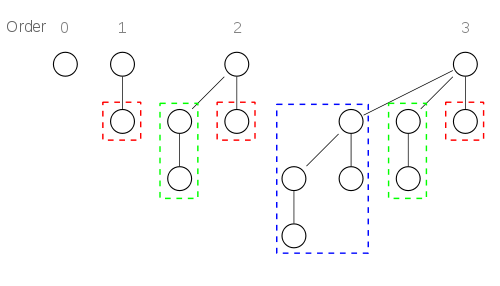
\includegraphics{images/binomial_tree.png}
                    \caption{Sample Binomial Heaps}
                    \label{fig:binomial_heap}
                \end{figure}

                There are a few properties of Binomial Heaps we know about\footnote{All properties in this list can be proved by induction.}:
                \begin{description}
                    \item[Size] of a $B_k$ is $2^k$.
                    \item[Height] of a $B_k$ is $k$, defined in the number of edges from the root to a leaf vertex.
                    \item[Width of level] $i$ of a $B_k$ is $ {k \choose i})$.

                        This is since ${k \choose i} = {{k-1} \choose i} + {{k-1} \choose {i-1}}$
                \end{description}
            % section binomial_tree (end)
            \section{Binomial Heaps} % (fold)
            \label{sec:binomial_heaps}
                To create binomial trees of arbitrary heights, we need to start using forests of binomial trees.

                We can represent $n = 13 = 0b1101 = 2^0 + 2^2 + 2^3$ elements as a $B_0$, $B_2$, and a $B_3$.

                In general, for $n$ elements, use $\log n$ trees.

                Most of our operations on this will be through a series of merges.

                \begin{description}
                    \item[Merge] works like binary addition ($\theta(1)$) across the trees, so the cost is the same as the bit cost of addition - $\theta(\log n)$
                    \item[Insert] is a merge of the pre-existing forest and a $B_0$ tree - $\theta(\log n)$ worst-case\footnote{TODO: is the amortized time different?}
                    \item[Delete Minimum] is done by finding the smallest tree, breaking removing the root vertex, and merging those to the remaining untouched trees - $\theta(\log n)$
                    % TODO: am I using the right names in the Decrease Key operation?
                    \item[Decrease Key] is done inside a binomial tree as a standard ``bubble up'', so the effect is limited to the height of the individual - $\theta(\log n)$
                    \item[Build Binomial Heap] can be done by repeated insertion in $O(n)$ time.
                    % TODO: how?
                \end{description}
            % section binomial_heaps (end)
        % chapter binomial_heaps (end)
        \chapter{Amortized Analysis} % (fold)
        \label{cha:amortized_analysis}

            \section{Example For Binomial Heaps} % (fold)
            \label{sec:example_for_binomial_heaps}
                Binomial heaps take $O(\log n)$ time to merge.
                Let's prove that.

                We want to determine the bit cost for incrementing a binary counter from $0$ to $n$.

                \subsection{Worst-Case Analysis} % (fold)
                \label{sub:worst_case_analysis}
                    The worst-case cost of one increment on a $k$-bit counter is $k$, so $n$ increments cost $O(n \log n)$ ($\log n$ bits flipped $n$ times).
                % subsection worst_case_analysis (end)
                \subsection{Amortized Analysis} % (fold)
                \label{sub:amortized_analysis}
                    We can get a better bound.
                    \begin{itemize}
                        \item The $2^0$ bit flips every time - $n$
                        \item The $2^1$ bit flips every other time - $\frac{n}{2}$
                        \item The $2^2$ bit flips every 4th time - $\frac{n}{4}$
                        \item etc.
                    \end{itemize}
                    The total cost is:
                    \begin{align*}
                        \sum_{i=0}^k \frac{n}{2^i} \le 2n
                    \end{align*}
                    Thus, the average cost of incrementing a counter is $\frac{2n}{n} = 2$.

                    Since binomial heap appending is representable with a bit cost of a binary counter, the total cost for making a binomial heap is $O(n)$.
                % subsection amortized_analysis (end)
            % section example_for_binomial_heaps (end)
            \section{An Amortized Definition} % (fold)
            \label{sec:an_amortized_definition}
                Given a sequence of $m$ operations with total cost $T(m)$, then the \textbf{amortized cost} per operation is $\frac{T(m)}{m}$.
            % section an_amortized_definition (end)
            \section{Potential Method for Amortized Analysis} % (fold)
            \label{sec:potential_method_for_amortized_analysis}
                The idea for this method is that we are keeping an account of (time) cost.

                Keeping track of a ``potential-time'' bank account, we keep track of the amortized difference between true \uline{cost} of operations and a \uline{charge} expected for all operations.

                We call the bank balance after the $i$th operation $\Phi_i$.

                \begin{itemize}
                    \item Cost is true.
                    \item Charge is artificial.
                \end{itemize}

                \begin{align*}
                    \Phi_i &= \Phi_{i-1} + \text{charge}(i) - \text{cost}(i)
                \end{align*}
                Since the potential ($\Phi_i$) and charge are artificial, we define them to make analysis easy.

                It's much simpler to define potential to get the charge:
                \begin{align*}
                    \text{charge}(i) &= \text{cost}(i) + \Phi_i - \Phi_{i-1}
                \end{align*}

                If the final potential is $\ge$ than the initial potential, then the amortized cost is $\le$ max charge.

                \begin{align*}
                    \sum_{i=1}^m \text{charge}(i) &= \sum_{i=1}^m \text{cost}(i) + \sum_{i=1}^m \Phi_i - \sum_{i=0}^{m-1} \Phi_i \\
                    &= \sum_{i=1}^m \text{cost}(i) + \Phi_m - \Phi_0 \\
                    \Phi_m - \Phi_0 \ge0 &\implies \sum \text{charge}(i) \ge \sum \text{cost}(i) \\
                    \text{amortized cost} &= \sum \frac{\text{cost}(i)}{m} \\
                    &\le \sum \frac{\text{charge}(i)}{m} \\
                    &\le \text{max charge}
                \end{align*}

                \subsection{Potential Analysis in a Nutshell} % (fold)
                \label{sub:potential_analysis_in_a_nutshell}
                    We need to invent a $\text{potential}(i)$ and a $\text{charge}(i)$ and prove that $\Phi_m \ge \Phi_0$.

                    A goal when inventing potential and charge is to prove that max charge is small, since the amortized cost is less than or equal to the maximum charged.

                    \begin{align*}
                        \text{charge}(i) &= \text{cost}(i) + \Phi_i - \Phi_{i-1}
                    \end{align*}
                % subsection potential_analysis_in_a_nutshell (end)
                \subsection{Binary Counters Using the Potential Method} % (fold)
                \label{sub:binary_counters_using_the_potential_method}
                    We know that only one bit will undergo $0 \to 1$ in a given increment.

                    The cost is high when $1 \to 0$ occurs many times.
                    Let's pay for $0 \to 1$ and an extra \$1 for when this bit eventually flips $1 \to 0$.

                    Thus, $\text{charge}(i) = 2$.

                    By theorem, the amortized cost $\le$ max charge $=2$, so long as $\Phi_m \ge \Phi_0$.

                    Formally, we'd like to specify the relation between $\text{charge}(i)$ and $\Phi_i$.

                    We make a jump here that $\Phi_i$ is the number of $1$s in the counter after the $i$th operation.

                    Supposing the $i$th operation changes $t_i$ bits $1\to0$, and $1$ bit $0\to1$.

                    Then we have:
                    \begin{align*}
                        \text{cost}(i) &= t_i + 1 \\
                        \Phi_i &= \Phi_{i-1} - t_i + 1 \\
                        \text{charge}(i) &= \text{cost}(i) + \Phi_i - \Phi_{i-1} \\
                        &= t_i + 1 - t_i - 1 \\
                        &= 2
                    \end{align*}

                    Thus, $\Phi_0 = 0$, and $\Phi_m \ge 0$, so the theorem applies.
                % subsection binary_counters_using_the_potential_method (end)
            % section potential_method_for_amortized_analysis (end)
            \section{Mergeable Heaps} % (fold)
            \label{sec:mergeable_heaps}
                There's a family of heaps who's main operation is a \verb|merge|.

                \begin{table}[h]
                    \centering
                    \begin{tabular}{ l | c | c | c }
                        & Binomial Heap & Lazy Binomial Heap & Fibonacci Heap \\ \hline \hline

                        insert          & $O(\log n)$   & {\color{BlueGreen}$O(1)$}    & $O(1)$            \\ \hline
                        delete min      & $O(\log n)$   & A $O(\log n)$     & A $O(\log n)$     \\ \hline
                        merge           & $O(\log n)$   & {\color{BlueGreen}$O(1)$}    & $O(1)$            \\ \hline
                        decrease key    & $O(\log n)$   & $O(\log n)$       & {\color{BlueGreen}A $O(1)$}  \\ \hline
                        build           & $O(n)$        & $O(n)$            & $O(1)$            \\
                    \end{tabular}
                \end{table}

                \subsection{Lazy Binomial Heaps} % (fold)
                \label{sub:lazy_binomial_heaps}
                    We can improve merge an insert by lazily combining trees during \verb|insert| and \verb|merge| operations.
                    We catch up on work when performing a \verb|delete min| operation to have exactly one tree of each rank.

                    \subsubsection{Implementing Delete-Min} % (fold)
                    \label{ssub:implementing_delete_min}
                        \begin{itemize}
                            \item Look at all roots to find the min
                            \item Delete that root, its children become separate
                            \item Consolidate ranks from smallest to largest
                        \end{itemize}
                        The wost case cost of \verb|delete min| is $\theta(n)$, with $n$ singleton trees.
                    % subsubsection implementing_delete_min (end)
                    \subsubsection{Amortized Analysis of Delete Min} % (fold)
                    \label{ssub:amortized_analysis_of_delete_min}
                        We theorize that Lazy Binomial Heaps have A $O(\log n)$ cost for \verb|delete min|.

                        By \textit{magic}, we pick $\Phi$ to represent the number of trees.
                        Thus, $\Phi_0 = 0$, and $\Phi_m \ge 0$, so $\Phi_m \ge \Phi_0$.

                        We know that $\text{charge}(i) = \text{cost}(i) + \Phi_i - \Phi_{i-1}$.
                        Let's examine other operations costs first:
                        \begin{itemize}
                            \item Merge cost is $O(1)$, since the number of trees is the same.
                            \item Decrease key cost is $O(\log n)$, and the number of trees is the same.
                            \item Insert cost is $O(1)$, since the number of trees increase by one.
                        \end{itemize}
                        In the case of \verb|delete min|, we have the degree $r \in O(\log n)$ of the node being deleted, and $t = \Phi_{i-1}$ as the number of trees being deleted.

                        Consolidate is called on $t-1+r$ trees.

                        Thus the total cost is $t - 1 + r + O(\log n)$.

                        After consolidation, we have $\Phi_i \in O(\log n)$.
                        \begin{align*}
                            \text{amortized cost} &\le \text{max charge} \\
                            &\le \text{cost}(i) + \Phi_i - \Phi_{i-1} \\
                            &= t - 1 + r + O(\log n) - t \\
                            &\le r + O(\log n) \\
                            r \in O(\log n) &\implies \text{amortized cost} \in O(\log n)
                        \end{align*}
                        Thus \verb|delete min| for lazy binomial heaps runs in $O(n)$ worst case, but $O(\log n)$ amortized.
                    % subsubsection amortized_analysis_of_delete_min (end)
                % subsection lazy_binomial_heaps (end)
                \subsection{Fibonacci Heaps} % (fold)
                \label{sub:fibonacci_heaps}
                    In these heaps, we want to improve the amortized cost of \verb|decrease key|.

                    What if instead of bubbling up, we simply ``cut off'' the node being decreased (and its sub-tree) from its parents?

                    This is dangerous, since the number of trees increases, and the number of child nodes change (not just $2^i$) for details.

                    TODO: the notes in lecture 3 reference assignment 2 for a practical alternative to Fibonacci Heaps. Dig this up.
                % subsection fibonacci_heaps (end)
            % section mergeable_heaps (end)
        % chapter amortized_analysis (end)
        \chapter{Splay Trees} % (fold)
        \label{cha:splay_trees}
            In a nutshell, splay trees are self-adjusting data structures that alter data structure after each query.
            They're the tree equivalent to lists that use \href{move-to-front}{https://en.wikipedia.org/wiki/Move-to-front\_transform} to improve lookup times.

            \section{Requisite Knowledge} % (fold)
            \label{sec:requisite_knowledge}
                \subsection{Dictionaries} % (fold)
                \label{sub:dictionaries}
                    These use keys from a totally ordered universe.
                    Operations include:
                    \begin{itemize}
                        \item Insert
                        \item Delete
                        \item Search
                    \end{itemize}

                    \subsubsection{Unbalanced Binary Search Trees} % (fold)
                    \label{ssub:unbalanced_binary_search_trees}
                        All operations take $O(h)$, where $h$ is the height of the tree.
                    % subsubsection unbalanced_binary_search_trees (end)
                    \subsubsection{Balanced Binary Search Tree} % (fold)
                    \label{ssub:balanced_binary_search_tree}
                        We limit $h \in O(\log n)$.
                        There are two (main) implementations: AVL and red-black trees.
                        Both implementations must keep the balance information, and are re-balanced using rotations.
                    % subsubsection balanced_binary_search_tree (end)
                % subsection dictionaries (end)
            % section requisite_knowledge (end)
            \section{Regarding Splay Trees} % (fold)
            \label{sec:regarding_splay_trees}
                Splay trees were invented (discovered?) by Sleator and Tarjan in `85.
                They offer A $\theta(\log n)$ cost per operation, with a $\theta(n)$ worst case running time.
                By not keeping balance information, they become easier to implement than other conventional balanced trees.

                % TODO: This is actually an exercise. Find the example.
                The course notes allude to an example where single rotations do not give good average behavior, so we will do double rotations instead.

                \subsection{Splay Operation} % (fold)
                \label{sub:splay_operation}
                    The \verb|splay(x)| operation moves $x$ repeatedly to the root.
                    This occurs through three cases.
                    Refer to Figures \ref{fig:splay_trees_case_1}, \ref{fig:splay_trees_case_2}, and \ref{fig:splay_trees_case_3}.
                    \begin{figure}[h]
                        \centering
                        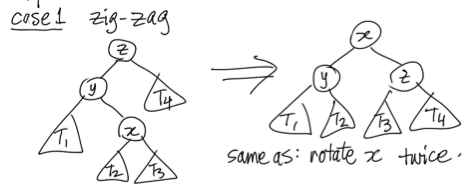
\includegraphics{images/splay_trees_case_1.png}
                        \caption{Splay Trees Case 1}
                        \label{fig:splay_trees_case_1}
                    \end{figure}
                    \begin{figure}[h]
                        \centering
                        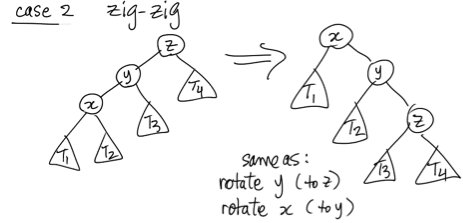
\includegraphics{images/splay_trees_case_2.png}
                        \caption{Splay Trees Case 2}
                        \label{fig:splay_trees_case_2}
                    \end{figure}
                    \begin{figure}[h]
                        \centering
                        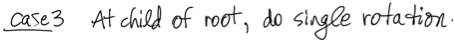
\includegraphics{images/splay_trees_case_3.png}
                        \caption{Splay Trees Case 3}
                        \label{fig:splay_trees_case_3}
                    \end{figure}
                % subsection splay_operation (end)
                \subsection{Splay Tree Methods} % (fold)
                \label{sub:splay_tree_methods}
                    \begin{description}
                        \item[Search] - after finding $x$, calling \verb|splay(x)|, even for unsuccessful searches.
                        \item[Insert] - usual binary search tree insert, then we \verb|splay| the new node.
                        \item[Delete] - usual binary search tree delete, then splay the parent of the node being removed.
                    \end{description}
                % subsection splay_tree_methods (end)
            % section regarding_splay_trees (end)
            \section{Amortized Analysis of Splay Trees} % (fold)
            \label{sec:amortized_analysis_of_splay_trees}
                If the height $h$ of a tree is large, then search is expensive, and we pay out of potential.

                We define $D(x)$ as the number of descendants of $x$, including $x$, and $r(x) = \log(D(x))$ .
                Finally, we define $\Phi(T) = \sum_x r(x)$.
                By \textit{magic}, we have the max as $\Phi_{\text{max}} = O(\log(n!)) = O(n\log(n))$, and the min as $\Phi_\text{min} = O(n)$.

                For a single node, we call $r(x)$ the current rank, and $r'(x)$ the rank after calling \verb|splay(x)|.

                We claim that the amortized cost of one step of \verb|splay(x)| is:
                \begin{align*}
                    O(\text{splay}(x)) &\le
                    \left\{
                        \begin{array}{lr}
                            3 (r'(x) - r(x)) :& \text{ for cases 1 and 2}\\
                            3 (r'(x) - r(x)) + 1 :& \text{ for case 3}
                        \end{array}
                    \right.
                \end{align*}
                Note that $(r''(x) - r'(x)) + (r'(x) - r(x)) = r''(x) - r(x)$.

                Since $\Phi_i \ge \Phi_0$, we now want to find the amortized cost.

                \begin{itemize}
                    \item For case 3, refer to Figure~\ref{fig:splay_trees_amortized_case_3}.
                        \begin{figure}[h]
                            \centering
                            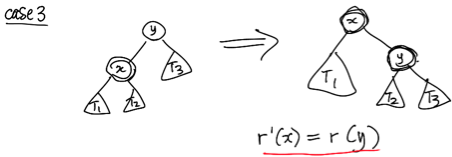
\includegraphics{images/splay_trees_amortized_case_3.png}
                            \caption{Amortized Splay Tree Analysis - Case 3}
                            \label{fig:splay_trees_amortized_case_3}
                        \end{figure}
                        \begin{align*}
                            \text{amortized cost} &\le \text{charge} \\
                            &= \text{true cost} + \text{change in potential} \\
                            &= 1 + r'(x) + r'(y) - r(x) - r(y) \\
                            r'(x) = r(y) &\implies \text{amortized cost} = 1 + r'(y) - r(x) \\
                            &\le 1 + r'(x) - r(x) \\
                            &\le 1 + 3(r'(x) - r(x))
                        \end{align*}
                    \item For case 1, refer to Figure~\ref{fig:splay_trees_amortized_case_1}.
                        \begin{figure}[h]
                            \centering
                            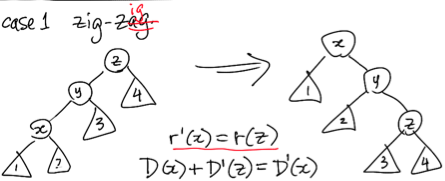
\includegraphics{images/splay_trees_amortized_case_1.png}
                            \caption{Amortized Splay Tree Analysis - Case 1}
                            \label{fig:splay_trees_amortized_case_1}
                        \end{figure}
                        \begin{align*}
                            \text{amortized cost} &\le \text{true cost} + \text{change in potential} \\
                            &= 2 + (r'(x) + r'(y) + r'(z) - r(x) - r(y) - r(z)) \\
                            r'(x) = r(z) &\implies \text{amortized cost} \le 2 + r'(y) + r'(z) - r(x) - r(y) \\
                            r'(y) \le r'(x) \land -r(y) \le -r(x) &\implies \text{amortized cost} \le 2 + r'(x) + r'(z) - 2r(x)
                        \end{align*}
                        To show that $2 + r'(x) + r'(z) - 2r(x) \le 3(r'(x) - r(x))$, it is enough to show that $2 \le 2r'(x) - r(x) - r'(z)$.

                        \begin{align*}
                            \forall x, y > 0 \land x+y \le 1 &: \text{Range}(\log x + \log y) = (-\infty, -2] \\
                            \implies \forall a + b \le c &\to \log{\left(\frac{a}{c}\right)} + \log{\left(\frac{b}{c}\right)} \le -2 \\
                            D(x) + D'(z) \le D'(x) &\implies \log(D(x)+ \log(D'(z)) \le 2 \log(D'(x)) - 2 \\
                            r(x) + r'(z) &\le 2r'(x) - 2 \\
                            2 &\le 2r'(x) - r(x) - r'(z)
                        \end{align*}
                        Thus the amortized cost of case 1 is $\le 3(r'(x) - r(x))$.
                    \item Case 2 is incredibly similar to case 1 with minor (ordering) modifications.
                \end{itemize}
                Without proof\footnote{scraig postulates that this can be proved with a telescoping sum}, we claim that a tree $T$ root $t$ and node $x$, the amortized cost of \verb|splay(x)| is:
                \begin{align*}
                    A O(\text{splay}) &\le 3(r(t) - r(x)) + 1 \\
                    &\in O(\log{\frac{D(t)}{D(x)}}) \\
                    &= O(\log n)
                \end{align*}

                Let $r_i = r(x)$ after the $i$th step of the splay.
                So $r_0 = r(x)$, and $r_k = r(t)$ (where $k$ is the final step).
                Thus the overall amortized cost of splay is:
                \begin{align*}
                    A O(\text{splay}) &= 1 + \sum_{i=1}^{k} 3(r_i - r_{i-1}) \\
                    &= 3(r_k - r_0) + 1
                \end{align*}

                We know that the cost of walking down the tree in each operation is $\le$ the cost of the ensuing splay.
                Thus, we know the amortized cost of \verb|insert|, \verb|search|, and \verb|delete| in a splay tree is $O(\log n)$.

                We briefly touched in class that \verb|insert| and \verb|delete| both modify potential, but this is still covered by the $\log n$ work to walk to the inserted and deleted value.
            % section amortized_analysis_of_splay_trees (end)
        % chapter splay_trees (end)
        \chapter{Union-Find Problem} % (fold)
        \label{cha:union_find_problem}
            Connected components in a graph are essentially the components where two can reach each other.

            We want to find all connected components, and identify which component a given vertex is in.
            Let's make this efficient.

            In general, we assume we are given a graph $G$ with $n$ vertexes and $m$ edges.
            We then need to respond to two queries:
            \begin{description}
                \item[find] are vertexes $a$ and $b$ in the same component?
                \item[union] connect the components which vertexes $c$ and $d$ lie in.
            \end{description}

            Using depth-first search, it takes $O(n+m)$ time to perform \verb|find|, and $O(1)$ time to perform \verb|union|.

            \section{Dynamic Graph Connectivity} % (fold)
            \label{sec:dynamic_graph_connectivity}
                For many data structures, we can get much faster runtime by maintaining (and later updating) results as the underlying data changes.

                Examples of where this is useful:

                \begin{itemize}
                    \item Social networks as relationships are added and deleted.
                    \item Minimum spanning tree\footnote{This is a special case of \textbf{Incremental Dynamic Connectivity}.}
                    \item Kruskal's Algorithm\footnote{
                        Greedy algorithm that orders edges by weight, then adds them slowly into a tree (if an edge creates a cycle, don't add it).
                        We end up with a minimum spanning tree.}
                \end{itemize}
            % section dynamic_graph_connectivity (end)
            \section{Union-Find Data Structure} % (fold)
            \label{sec:union_find_data_structure}
                We want to maintain a collection of disjoint sets then evaluate:
                \begin{description}
                    \item[Union$(A, B)$] unites (modifies) the two sets $A$ and $B$ to be in the same set.
                    \item[Find$(e)$] which set contains $e$?
                \end{description}

                If we analyze Kruskal's algorithm using union-find data structure, we get:
                \begin{align*}
                    \mbox{sort} + 2m \mbox{Finds} + n \mbox{Unions}
                \end{align*}
                Sort takes $O(m \log m) = O(m \log n)$ time\footnote{Since $m \le n^2$, we have $O(\log m) = O(\log n)$}, so we want the finds and unions to work in $\le O (m \log n)$ to have a speedy algorithm.

                Define $n$ as the number of elements, and $m$ as the number of operations.
                For all implementations, the number of unions $\le n - 1$.
                \subsection{Implementation With an Array} % (fold)
                \label{sub:implementation_with_an_array}
                    Using an array $S[1...n]$, where $S[i]$ contains the name of a set containing $i$.
                    \begin{description}
                        \item[Find] $O(1)$
                        \item[Union] $O(n)$ worst case
                    \end{description}

                    To make this marginally faster, we can maintain a set for each set as well.
                    Thus, \verb|union(A, B)| will update $S$ for the smaller set.
                    Since each element changes its set name $\le \log n$ times, the overall cost of all unions is $\le O(n \log n)$.

                    The cost of $m$ operations is thus $O(m + n \log n)$.
                    With this implementation, this is the best possible if the number of finds is $\Omega(n \log n)$.

                    Thus in this case, we get $O((n+m) \log n)$ for Kruskal's algorithm.
                % subsection implementation_with_an_array (end)
                \subsection{A Better Implementation} % (fold)
                \label{sub:a_better_implementation}
                    In the case that the number of finds is small, the array-based union-find implementation is horrible.

                    When we represent each set as a tree, life becomes much better.

                    \begin{description}
                        \item[Union] is implemented as merging the smaller tree as a child to the root of the larger tree.
                            See Figure~\ref{fig:union_find_union} for a pictorial visualization.
                        \item[Find] is implemented by traversing up the tree from the node, then returning the name of the root node.
                            After traversing upwards, we perform path compression by setting the parent of all vertexes in the path to be the root of this tree.
                            See Figure~\ref{fig:union_find_find} for a pictorial visualization.
                    \end{description}
                    \begin{figure}[h]
                        \centering
                        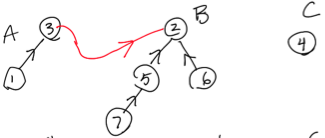
\includegraphics{images/union_find_union.png}
                        \caption{``Union'' Operation in the Union-Find Data Structure}
                        \label{fig:union_find_union}
                    \end{figure}
                    \begin{figure}[h]
                        \centering
                        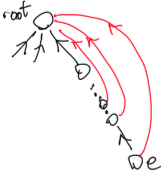
\includegraphics{images/union_find_find.png}
                        \caption{``Find'' Operation in the Union-Find Data Structure}
                        \label{fig:union_find_find}
                    \end{figure}
                    We determine the smaller tree by keeping track of the ``rank'' of a tree - the height if there was no path compression.
                    When \verb|union|-ing a smaller $r_2$ onto a larger $r_1$, the the new rank is $\max\{r_1, r_2+1\}$.
                % subsection a_better_implementation (end)
            % section union_find_data_structure (end)
            \section{Analysis of the Union-Find Data Structure} % (fold)
            \label{sec:analysis_of_the_union_find_data_structure}
                The implementation is simple, but the analysis is hard.
                In `75, Tarjan proved that the cost of $m$ operations is $\Theta(m \alpha(m, n))$ time\footnote{$\alpha(m, n)$ is the inverse Ackerman function. It is very slow growing, and is $\le 5$ for all practical purposes.}.

                We will prove the slightly higher bound of $O(m \log^* n)$ time for $m$ operations\footnote{$\log^* n$ is essentially the minimum number of times $log(n)$ needs to be recursively called in order for $\log(\log(\ldots(n))) \le 1$. The inverse of this is $2\uparrow n$, which is $2$ exponentiated with itself $n$ times.}.

                We know that the cost of \verb|find(v)| is the same as the distance from $v$ to the root.
                In a nutshell, we will charge some to the \verb|find|, and some to the nodes along the path from $v$ to the root, then sum it up.

                We claim (without proof) that:
                \begin{enumerate}
                    \item $\text{rank}(v) < \text{rank}(\text{parent}(v))$.
                    \item The number of vertexes of rank $r$ is $\le \frac{n}{2^r}$ in size\footnote{This is because a vertex of rank $v$ has $n \ge 2^r$ descendants, and vertexes of rank $r$ have disjoint descendants.}.
                \end{enumerate}

                In our analysis, we divide vertexes into groups based on their rank.
                A vertex of rank $r$ goes in a group number $\log^*(r)$.
                Thus a group $g$ contain the ranks $2\uparrow(g-1) + 1, 2\uparrow(g-1) + 2, \ldots, 2\uparrow g$.
                For group $g$, the number different ranks $c(g)+1$ in $g$ is $\le 2 \uparrow g$.

                Since the largest rank in a structures can be $n$, the number of groups must be $\le \log^* n$.

                We want to find the charge for \verb|find(v)|:
                For each vertex $u$ on the path from $v$ to the root:
                \begin{itemize}
                    \item if $u$ has a parent and grandparent, and $\text{group$(u)$} = \text{group$(\text{parent$(u)$})$}$, then charge 1 to $u$.
                    \item Otherwise, charge 1 to \verb|find(v)|.
                \end{itemize}
                Thus the total charge to $\text{find$(v)$} \le \log^* n + 1$, since the group changes $\le \log^*n - 1$ times, and $2$ more for the root and it's child.

                We now need to determine the charge to individual nodes.

                If a vertex $u$ in group $g$ is charged, then path compression will give it a new parent of higher rank.
                Therefore a $u$ in group $g$ is charged $c(g)$ times until its parent is in a higher group.
                We know that $c(g) \le 2 \uparrow g$.

                The total charge to all nodes in a group $g$ is:
                \begin{align*}
                    (\text{number of ranks in $g$})(\text{number of nodes in $g$}) &= c(g)N(g) \\
                    N(g) &\le \sum_{r = 2\uparrow(g-1)+1}^{2 \uparrow g} \frac{n}{2^r} \\
                    &\le \frac{n}{2^{2 \uparrow(g-1)+1}} \sum_{i=0}^\infty \frac{1}{2^i} \\
                    &\le \frac{n}{2 \uparrow g} \\
                    \implies c(g)N(g) &\le n
                \end{align*}
                Thus the total charge to all nodes is $n \log^* n$.

                For Kruskal's algorithm, we find the total charge to \verb|finds| and \verb|nodes| as:
                \begin{align*}
                    O(m (\log^*n + 1) + n \log^* n) &= O(m \log^* n)
                \end{align*}
                Not bad.
            % section analysis_of_the_union_find_data_structure (end)
        % chapter union_find_problem (end)
        \chapter{Geometric Data Structures} % (fold)
        \label{cha:geometric_data_structures}
            So far data structures have been implemented with comparable keys.

            When working in higher dimensions, we have two main problem types:
            \begin{itemize}
                \item Find points inside a region
                \item Find regions containing a point
            \end{itemize}
            \section{Range Search} % (fold)
            \label{sec:range_search}
                By preprocessing $n$ points in $k$ dimensions, so we can handle range queries.
                In 2D, this would be querying for points contained within a rectangle.

                We have 3 main measures for range search methods:
                \begin{description}
                    \item[P] the preprocessing time
                    \item[S] the space taken for preprocessing
                    \item[Q] the query time
                    \item[U] the update time (only some algorithms can have updated data)
                \end{description}
                \subsection{Range Queries for $k=1$} % (fold)
                \label{sub:range_queries_for_k_1}
                    When $k=1$, we sort data and use binary searches.
                    Thus we have:
                    \begin{description}
                        \item[P] $O(n \log n)$
                        \item[S] $O(n)$
                        \item[Q] $O(\log n + t)$, where $t$ is the output size.
                        \item[U] $O(\log n)$
                    \end{description}
                % subsection range_queries_for_k_1 (end)
                \subsection{Range Queries for $k=2$} % (fold)
                \label{sub:range_queries_for_k_2}
                    We have a few cool implementations, most of which are covered in CS240.

                    \subsubsection{Quad Tree} % (fold)
                    \label{ssub:quad_tree}
                        Divide squares into four subsquares, repeat until each square has $(0, 1)$ points.
                    % subsubsection quad_tree (end)
                    \subsubsection{$k$d-Tree} % (fold)
                    \label{ssub:kd_tree}
                        Divide points in half vertically then horizontally (then recurse).
                        \begin{description}
                            \item[P] $O(n \log n)$
                            \item[S] $O(n)$
                            \item[Q] $\Theta(\sqrt{n} + t)$, where $t$ is the output size.
                        \end{description}
                    % subsubsection kd_tree (end)
                    \subsubsection{Range Trees} % (fold)
                    \label{ssub:range_trees}
                        See the subsection on Range trees below.
                    % subsubsection range_trees (end)
                % subsection range_queries_for_k_2 (end)
                \subsection{Range Trees for $k=2$} % (fold)
                \label{sub:range_trees_for_k_2}
                    A $n$th dimension range tree improves $Q$ at the expense of $S$.
                    It uses a binary search tree across one dimension, where each internal node has an additional $n-1$-dimension range tree.

                    A $k=1$-dimension range tree is a sorted list.

                    \begin{description}
                        \item[P] sort by $x$, then sort by $y$ and do some work - $O(n \log n)$
                        \item[S] each point occurs in $\log n$ of the sorted-by-$y$ lists - $O(n \log n)$
                        \item[Q] search for the $x_l$ and $x_r$ in $O(\log n)$ time. For all children of paths to $x_l$ and $x_r$, we search the $y$ list - $O(\log^2 n + t)$
                    \end{description}

                    \subsubsection{Fractional Cascading} % (fold)
                    \label{ssub:fractional_cascading}
                        We can improve $Q$ to $O(\log n + t)$ by using a technique called fractional cascading.

                        Generally, we keep a pointer from each element in the $x$'s list to the corresponding element in $y$'s list.
                        This gives us $Q = (\log n + t)$, since we binary search \uline{once} for $y_U, y_L$ in the list of root and follow pointers.
                    % subsubsection fractional_cascading (end)
                % subsection range_trees_for_k_n (end)
            % section range_search (end)
            \section{Point Location} % (fold)
            \label{sec:point_location}
                Given a set of disjoint regions in a $k$-dimensional space, we want to quickly respond to queries that query the location they are in.
                This can help with queries like: which city is coordinate $(a,b)$ in?
                Where is the nearest Tim Hortons?
                etc.

                \subsection{Point Location for $k=1$ Dimension} % (fold)
                \label{sub:point_location_for_k_1_dimension}
                    In $1$d, we use a balanced binary search tree.
                    \begin{description}
                        \item[P] $O(n \log n)$
                        \item[S] $O(n)$
                        \item[Q] $O(\log n)$
                    \end{description}
                % subsection point_location_for_k_1_dimension (end)
                \subsection{Point Location for $k=2$ dimensions} % (fold)
                \label{sub:point_location_for_k_2_dimensions}
                    We can divide the entire space into slabs by adding a vertical line at every point.

                    Then given a query point $x$, find the correct slab ($O(\log n)$) then binary search by $y$ ($O(\log n)$).
                    \begin{description}
                        \item[Q] $O(\log n)$
                        \item[S] $\Theta(n^2)$ (ew)
                    \end{description}
                    \subsubsection{Less Space Through Persistent Data Structures} % (fold)
                    \label{ssub:less_space_through_persistent_data_structures}
                        Given that in one slab to the next, very few changes, we only need to make a BST for the leftmost slab and update for subsequent slabs.

                        The total number of updates to the BST is $O(n)$, since every segment is inserted and deleted exactly once.

                        If we update a BST and search it in the past, this idea is called a ``persistent data structure''.

                        \begin{description}
                            \item[Partial persistence] allows queries in the past and only the present be changed.
                            \item[Full persistence] allows queries and changes at any point in time.
                        \end{description}

                        Using Driscoll, \ldots, Tarjan `89, we can add partial persistence to any data structure.

                        This gives us a planar point location of:
                        \begin{description}
                            \item[P] $O(n \log n)$
                            \item[S] $O(n)$
                            \item[Q] $O(\log n)$
                        \end{description}
                        In an awesome way, this runs in the same time as the initial 1D problem.
                    % subsubsection less_space_through_persistent_data_structures (end)
                % subsection point_location_for_k_2_dimensions (end)
            % section point_location (end)
        % chapter geometric_data_structures (end)
        \chapter{Randomized Algorithms} % (fold)
        \label{cha:randomized_algorithms}
            Algorithms that use random numbers have their \uline{output} and/or their \uline{runtime} depend on random numbers.
            This forces us to use amortized (expected) analysis.

            Practicaly speaking, it gets us easier and faster algorithms.
            Theoretically speaking, it's \open whether randomization helps for \p vs \np, but we'll see an example where it'll help a tiny bit.

            In previous classes, we've seen QuickSort\footnote{See the QuickSort details in Section ~\ref{sec:quicksort}} and SkipLists.

            We define randomized algorithms as ones that execute either method \verb|rand[1, ..., n]| or \verb|rand[0, 1]|, both of which run in $O(1)$ time\footnote{We can get the first method using the second.}.

            Thus, the running time for fixed input depends on random numbers - i.e.  a \uline{random variable}.

            A few definitions are necessary:
            \begin{description}
                \item[Sample Space] is the space of all possible outcomes (for fixed input).
                \item[Random Variables] map the sample space to real numbers (at runtime).
            \end{description}
            We need to rely on some stats for the upcoming parts.
            See Section~\ref{sec:expected_values_statistics} for expected knowledge.

            We set the function $T(I)$ as the time it takes depending on the random variable $I$.
            Obviously, we set $E(T(I))$ as the expected runtime across all possible values of $I$.

            We then say that the function\footnote{$I$ and $n$ are different types, and polymorphism works in pseudocode.}$T(n)$ is the maximum of $E(T(I))$ across all $I$'s.
            \begin{align*}
                T(n) &= \max_{|I| = n} E(T(I))
            \end{align*}
            \section{Selection} % (fold)
            \label{sec:selection}
                Given a set of $n$ numbers $S$, we'd like to return the $k$-th smallest element of $S$.

                For example:
                \begin{itemize}
                    \item $k = 1$ is the min
                    \item $k = 2$ is the 2nd min
                    \item $k = n$ is the max
                    \item $k = \myfloor{\frac{n}{2}}$ is the median
                \end{itemize}
                Let's implement QuickSelect:
                \begin{verbatim}
    def QuickSelect(S, k):
        n = |S|
        if n < constant
            Sort(S)
            return kth element
        i = rand(1...n)
        partion S into:
        L = {s : s < S[i]}
        M = {s : s == S[i]}
        R = {s : s > S[i]}
        if k < |L| return QuickSelect(L, k)
        if k <= |L| + m return s[i]
        return QuickSelect(B, k - (|L| + |M|))
                \end{verbatim}
                This is worst-case $O(n^2)$ when pivot is always the min or the max, but it often isn't the worst-case.

                We can do more detailed analysis to find the expected time of finding it on a set $S$ of size $n$.

                In other words, we want $E(T(n))$, where $T(n)$ is a random variable runtime of QuickSelect on a set of size $n$.

                We have recursive calls on sets of size $\ell$ or $n - \ell$.
                For an upper bound, assume that $k$ lies in the larger (worse) half of the recursion.
                In other words, we assume that $k \le \frac{n}{4}$ or $k \ge \frac{3n}{4}$.
                Thus the recursion is $\le T(\frac{3n}{4})$.

                Assuming that $T(i) \le T(j)$ for $i \le j$, we get:
                \begin{align*}
                    E(T(n)) &\le \frac{1}{2}E\left(T\left(\frac{3n}{4}\right)\right) + \frac{1}{2}E\left(T\left(n - 1\right)\right) + O(n) \\
                    f\left(n\right) &\le \frac{1}{2}f\left(\frac{3n}{4}\right) + \frac{1}{2}f\left(n - 1\right) + O(n)
                \end{align*}
                We can prove by induction that $f(n) = O(n)$.
            % section selection (end)
            \section{Random V.S. Non-Randomized Algorithms} % (fold)
            \label{sec:random_v_s_non_randomized_algorithms}
            % TODO: put this in a table
                1960 Hoare QuickSelect has $3n + o(n)$ expected comparisons \\
                1973 BFPRT created a non-randomized selection in $O(n)$ time, with $5.43n + o(n)$ comparisons. This is the same with respect to $O(n)$, but different constant than randomized algorithms. \\
                1975 Floyd Rivest created a randomized algorithm that takes $1.5n + o(n)$ expected comparisons. \\
                1989 Munro \& Cunto proved that any ralgorithm takes at least $1.5n$ expected comparisons. \\
                1985 [???] proved a lower bound of $2n$ comparisons for non-randomized algorithms. Randomization probably helps. \\

                Currently, our best non-randomized bounds are:
                \begin{table}[h]
                    \centering
                    \begin{tabular}{ | l | l | l |}
                        \hline
                        Bound & Year & \# comparisons \\ \hline \hline
                        Upper Bound & 1999 & 2.95n \\ \hline
                        Lower Bound & 2001 & $(2 + \varepsilon) n$, $\varepsilon = 2^{-80}$ \\ \hline
                    \end{tabular}
                \end{table}
            % section random_v_s_non_randomized_algorithms (end)
            \section{Lower Bound on Median} % (fold)
            \label{sec:lower_bound_on_median}
                \textbf{Theorem:}\footnote{Blum et al. `75}
                Finding the median of $n$ elements takes $\ge 1.5n$ comparisons in the worst case.

                \textbf{Proof:}\footnote{This proof type is an adversary proof.}

                Let $L = \{\text{elements } < m\}$, and $M = \{\text{elements } > m\}$.
                So that each set has $\frac{n-1}{2}$ elements.

                We claim that the number of $L$ vs $H$ comparisons must be $\ge \frac{n-1}{2}$ in the worst case.

                We set it up so the adversary answers the comparisons that our algorithm queries.
                Our adversary consistently answers by ``setting'' elements to $L$ and $H$ at all times.\footnote{We're effectively trying to find the worst case scenario, played out by an adversary. Stick to the plot, foo!}
                We can now create an adversary strategy:
                \begin{verbatim}
def compare(x, y):
    if x and y have been seen before:
        return result of comparison
    if one of (x, y) have been seen:
        put the unseen one in the other set
    if neither are set:
        put x in L, y in H
                \end{verbatim}
                An adversary must stop when $\max(|L|, |H|) = \frac{n-1}{2}$, so they can force at most $\frac{n-1}{2}$ comparisons.

                Since there are always $\ge n-1$ $L$ vs $H$ comparisons, and the adversary can force an additional $\ge \frac{n-1}{2}$ $L$ vs $H$ comparisons, the overall algorithm must make $\ge 1.5n$ comparisons in the worst case.

                \subsection{$O(n)$ Non-Randomized Selection Algorithm} % (fold)
                \label{sub:on_non_randomized_selection_algorithm}
                    The idea here is that we divide sets of $n$ elements into groups of 5, then find the median of each group.
                    We then execute a recursive call to find a median of medians $P$.
                    This guarantees $P$ between $\frac{3n}{10}$ and $\frac{7n}{10}$ in rank.
                    We get the recurrence:
                    \begin{align*}
                        T(n) &= T\left(\frac{n}{5}\right) + T\left(\frac{7n}{10}\right) + O(n)
                    \end{align*}
                    We can prove that $T(n) = O(n)$.\footnote{This can probably be done using induction, but it isn't noted.}

                    For more information, look up the \href{https://en.wikipedia.org/wiki/Median_of_medians}{``median of medians''} algorithm online.

                % subsection on_non_randomized_selection_algorithm (end)
            % section lower_bound_on_median (end)
        % chapter randomized_algorithms (end)
        \chapter{Primality Testing} % (fold)
        \label{cha:primality_testing}
            \section{Randomized Algorithm Types} % (fold)
            \label{sec:randomized_algorithm_types}
                There are two kinds of randomized algorithms:
                \subsection{Las Vegas Type Algorithms} % (fold)
                \label{sub:las_vegas}
                    Las Vegas algorithms always return the correct output, and have good expected runtime.
                    An example of this type of algorithm is quicksort.

                    We can convert Las Vegas to Monte Carlo algorithms by stopping after some time and outputting a junk answer.
                % subsection las_vegas (end)
                \subsection{Monte Carlo Type Algorithms} % (fold)
                \label{sub:monte_carlo_type}
                    Monte Carlo algorithms are quick with a high probability of success, and have a good guaranteed runtime.

                    If we have a fast correctness test we can convert Monte Carlo algorithms to Las Vegas algorithms, repeating the algorithm if output isn't correct.
                % subsection monte_carlo_type (end)
            % section randomized_algorithm_types (end)
            \section{Primality Testing Using a Monte Carlo Algorithm} % (fold)
            \label{sec:primality_testing_using_a_monte_carlo_algorithm}
                Given an odd number $n$, is $n$ composite?\footnote{In other words, is $n$ not prime?}
                Phrased this way, we have a decision problem in \np, which is verifying \verb|YES| answers.

                It is important to know that while the input is $n$, the input size is $\log(n)$ -- the number of bits used expressing $n$.
                Thus trial division ($O(\sqrt{n})$ time) is not poly-time.\footnote{In 2002, Agrawal, Kayal, and Saxena published a poly-time non-randomized algorithm to test primality known as the \href{https://en.wikipedia.org/wiki/AKS_primality_test}{AKS Primality Test}.}

                We use the following theorem to help us with our solutions:
                \subsection{Fermat's Little Theorem} % (fold)
                \label{sub:fermat_s_little_theorem}
                    If $p$ is prime, then $\forall 0 < a < p$: $a^{p-1} \equiv 1 \mod p$.

                    We can prove this by showing:
                    \begin{align*}
                        a^p(p-1)! \equiv (p-1)! \mod p \\
                        a^p \equiv 1 \mod p
                    \end{align*}

                    The contrapositive\footnote{Contrapositive notes can be found at \ref{sub:contrapositive}.} states that whenever $a^{n-1} \not \equiv 1 \mod n$ doesn't hold for $0 < a < n$, then $a$ is a \textit{Fermat Witness} to $n$ being composite.
                    % TODO: elaborate on what the divisor of $n$ is in terms of $a$.
                % subsection fermat_s_little_theorem (end)
                \subsection{Prime-Testing} % (fold)
                \label{sub:prime_testing}
                    The idea is to test $n$ being composite using randomly-generated $a$ in $[1, \ldots, n-1]$ for being a Fermat witness.

                    If it is, then \textsc{yes} $n$ is composite.
                    If it isn't, then \textsc{maybe} $n$ is prime.

                    The bad news is that there are composite numbers \uline{without any} Fermat witnesses\footnote{The numbers without Fermat witnesses are called \uline{Carmichael numbers}.
                    The first $3$ are $561$, $1105$, $1729$.}.

                    Where $n-1 = 2^t u$ (for an odd $u$), we need a \uline{Strong Witness} that $n$ is prime.
                    We define $a \in [1, n-1]$ as a strong witness of $n$ being composite if for some $0 \le i < t$, $k = 2^i u$:
                    \begin{align*}
                        a^k \not \equiv 1 , -1 \mod n \\
                        a^{2k} \equiv 1 \mod n
                    \end{align*}
                    In CLRS, they prove that if $n$ is prime, there are no strong witnesses;
                    they also prove that if $n$ is composite, there are $\ge \frac{n-1}{2}$ strong witnesses.
                % subsection prime_testing (end)
                \subsection{Implementation} % (fold)
                \label{sub:implementation}
                    \begin{lstlisting}
witness (a , n):
u = n - 1 % 2
t = log((n - 1) / u) // base 2
x[0] =  a ^ u mod n
for i = 1 ... t:
    x[i] = x[i-1]^2 mod n
    if (x[i] == 1 and x[i-1] != 1 and x[i-1] != n - 1):
        return true // a is a strong witness to n being composite
return x[t] != 1 // a is a Fermat witness to n being composite
                    \end{lstlisting}
                    The runtime of this algorithm is polynomial in $\log n$.
                % subsection implementation (end)
                \subsection{Miller-Rabin Algorithm} % (fold)
                \label{sub:miller_rabin_algorithm}
                    The idea of this algorithm is to test $s$ times that random numbers aren't witnesses to $n$ being composite.
                    \begin{lstlisting}
isComposite(n):
    for i = 1 ... s:
        x = rand(1...n-1)
        if (witness(x, n)):
            return YES // n is composite
    return MAYBE // n is prime
                    \end{lstlisting}
                    If $n$ is prime, the algorithm is always correct.
                    IF $n$ is composite however, we can tabulate the probability it is unsure:
                    \begin{align*}
                        Pr\{ \text{Alg outputs \textsc{maybe}}\} &= Pr\left\{ \cap_{j=1}^s \left\{\text{at trial $j$, $x$ is not a strong witness } \right\} \right\} \\
                        &= \frac{1}{2^s}
                    \end{align*}
                    This is a Monte-Carlo algorithm with a \uline{one-sided error}\footnote{This means that for a decision problem, only one of \textsc{YES} or \textsc{NO} can be wrong.}.
                % subsection miller_rabin_algorithm (end)
            % section primality_testing_using_a_monte_carlo_algorithm (end)
            \section{Complexity Classes} % (fold)
            \label{sec:complexity_classes}
                We can define a number of decision classes:
                \begin{description}
                    \item[\p] are the decision problems solvable in polynomial time.
                        These are also known as the class of languages $L$ accepted in polynomial time.
                    \item[\np] are the class of languages $L$ accepted in non-deterministic polynomial time.
                        These are also known as the decision problems that can be \uline{verified} in polynomial time\footnote{i.e. the \textsc{yes} answers can be verified in poly-time.}.
                \end{description}
                There are a few\footnote{okay, maybe ``many''} \open problems about this\footnote{The classes \textsc{rp} and \textsc{co-np} are defined later.}: % TODO: Where is co-np?
                \begin{align*}
                    \np &\stackrel{?}{=} \textsc{co-np} \\
                    \p &\stackrel{?}{=} \np \\
                    \p &\stackrel{?}{=} \np \cup \textsc{co-np} \\
                    \p &\stackrel{?}{=} \textsc{rp} \\
                    \textsc{rp} &\stackrel{?}{=} \np
                \end{align*}
                \subsection{Randomized Polynomial Time, One Sided Monte-Carlo} % (fold)
                \label{sub:randomized_polynomial_time_one_sided_monte_carlo}
                    The \textsc{rp} class of problems is the class of languages that have a randomized algorithm $A$ running in worst-case polynomial time such that for any input $x$:
                    \begin{align*}
                        x \in L \implies Pr[\text{$A(x)$ accepts}] & \ge \frac{1}{2} \\
                        x \not \in L \implies Pr[\text{$A(x)$ accepts}] & = 0
                    \end{align*}
                    In other words, the algorithm always returns no for input $x$ that don't match, and \textit{sometimes} returns yes for $x$ that match
                    \footnote{Though the specification is that the probability must be $\ge 0.5$, repeated random tests can increase the probability for lower values. A better constraint is that the probability that $A(x)$ accepts must be non-zero.}.

                    We know that $\p \subseteq \textsc{rp}$, since the probabilities that \p problems will accept and decline are 0 and 1 respectively.

                    Supposing language $L$ is in \textsc{rp}, i.e. there is a randomized algorithm $A$ that fits the definitions of \textsc{rp}.
                    $A$ depends on $x$ and random choices.
                    If we think of the random choices as a string $y$ of random bits, we write $A(x, y)$ as applying $A$ on $x$ with random bits $y$.
                    Since $A$ runs in polynomial with respect to $|x|$ ($A \in p(|x|)$), we know that the string $y \in p(|x|)$.
                    Using $A$ as the verification algorithm and $y$ as the certificate, we can show that $L$ is in \np.
                % subsection randomized_polynomial_time_one_sided_monte_carlo (end)
                \subsection{Zero Error Probabilistic Polynomial Time} % (fold)
                \label{sub:zero_error_probabilistic_polynomial_time}
                    \textsc{zpp} is the class of languages accepted by Las Vegas algorithms with an expected polynomial runtime.

                    Note that $\p \subseteq \textsc{zpp} \subseteq \textsc{rp}$.

                    An in-class quiz consisted in proving that $\textsc{zpp} = \textsc{rp} \cap \text{co-}\textsc{rp}$ is true.

                    See \href{https://en.wikipedia.org/wiki/RP_(complexity)}{here for more details} on the co-\textsc{rp} complexity class.
                % subsection zero_error_probabilistic_polynomial_time (end)
                \subsection{Open Questions} % (fold)
                \label{sub:open_questions}
                    It is \open if these containments are proper, or if they can be made more precise:
                    \begin{align*}
                        \p \subseteq \textsc{rp} \subseteq \np
                    \end{align*}
                % subsection open_questions (end)
            % section complexity_classes (end)
        % chapter primality_testing (end)
        \chapter{Finger-Printing - Pattern Matching and Polynomial Identities} % (fold)
        \label{cha:finger_printing_for_pattern_matching_and_polynomial_identities}
            \section{String Equality} % (fold)
            \label{sec:string_equality}
                It's pretty expensive to compare strings, especially if they're long, stored in separate locations, etc.
                We compare a smaller fingerprint $x$ where $x$ is an $n$-bit binary number ($x < 2^n$).
                For a randomly chosen $p \in \{ 1 \ldots M \}$\footnote{$M$ is chosen later}, we can set:
                \begin{align*}
                    H_p (x) &= x \mod p
                \end{align*}
                While $x = y$ implies $H_p(x) = H_p(y)$, this contrapositive doesn't hold true if $p$ divides $|x - y|$.

                With repeated (in)equality testing of $H_p(x)$ to $H_p(y)$, we can build confidence about $x \stackrel{?}{=} y$.
                Our algorithm will know for sure when $x \ne y$, but it can't be sure they are equal.
                Thus this is a Monte-Carlo Algorithm.

                To better analyze our algorithm, we want to define $Pr\{\text{failure}\}$.
                If we define $\pi(n)$ as the number of primes less than $n$, then $\pi(n) \approx \frac{n}{\ln n}$\footnote{This is a prime number theorem.}.
                Another result from number theory dictates that the number of prime divisors of $A < 2^n$ is $\pi(n)$.
                \begin{align*}
                    Pr\{\text{failure}\} &= \frac{\text{number of primes $p < M$ and $p$ divides $|x-y| < 2^n$}}{\pi(M)} \\
                    &= \frac{\pi(n)}{\pi(M)}
                \end{align*}
                If we pick $M = n^2$, then we have $Pr\{\text{failure}\}$:
                \begin{align*}
                    Pr\{\text{failure}\} &= \frac{n}{\ln n} \frac{\ln n^2}{n^2} \\
                    &= \frac{2}{n}
                \end{align*}
                % TODO: this is so hand-wavy, it hurts.
            % section string_equality (end)
            \section{Pattern Matching} % (fold)
            \label{sec:pattern_matching}
                We can use a similar idea as string matching for pattern matching:

                Given a test string $T$ and a pattern string $P$ (where $|T| = n$, $|P| = m$), does $P$ appear as a substring of $T$?

                There's a straightforward $O(nm)$ solution\footnote{We have a few other methods:\\
                Using finite automata, we have $O(m|\Sigma| + n)$ non-randomized algorithms, where $\Sigma$ is the size of the alphabet. \\
                Using Knuth-Morris-Pratt or Boyer-Moore algorithms, we have $O(n+m)$ non-randomized algorithms.}.

                \subsection{Rabin-Karp Algorithm} % (fold)
                \label{sub:rabin_karp_algorithm}

                    \textbf{Rabin-Karp} supplies a simple and efficient randomized algorithm.

                    Suppose $T$ and $P$ are binary strings.
                    We want to compare the fingerprint of $P$ to fingerprints of successive substrings of $T$.

                    Using a ``rolling hash'', these fingerprints in $T$ can be computed very efficiently\footnote{$H_p(T[i+1 \ldots i+m]) = (2 H_p(T[i \ldots i+m - 1]) - T[i] 2^m + T[i + m]) \mod p $}.

                    \begin{lstlisting}
def hasMatch(text T, text P):
    p = randomPrime(1 ... m)
    compute Hp(P)
    compute Hp(T[1 ... m])
    for i in range(1 ... n-m+1):
        if Hp(P) == Hp(T[i ... i+m-1])
            return PROBABLE_MATCH
    output NO_MATCH
                    \end{lstlisting}
                    We have the runtime of $O(n + m)$ arithmetic operations.
                    We are more concerned about the failure rate - the probability that we output \textsc{Probable\_Match} without there being a real match.
                    Iff $p$ divides\footnote{Where $P$ and $T[\ldots]$ are viewed as binary numbers} $|P - T[i \ldots i+m -1]|$ for some $i$, then $p$ divides $\Pi_i |P - T[i \ldots i+m - 1] \le 2^{nm}$.

                    Thus, the following of failure is: (and to recap...)
                    \begin{align*}
                        & \text{$p$ divides } |P - T[i \ldots i + m - 1] \text{ for some $i$} \\
                        \implies & \text{$p$ divides } \Pi_i |P - T[i \ldots i + m - 1]| \le 2^{nm} \\
                        \implies & Pr\{ \text{failure} \} \le \frac{\pi(nm)}{\pi(M)}
                    \end{align*}
                    Where $M$ is some number.
                    We can choose $M = n^2 m$, then we have:
                    \begin{align*}
                        Pr\{\text{failure}\} &\le \frac{nm}{\ln (nm)} \frac{\ln(n^2 m)}{n^2 m} \\
                        &< \frac{2}{n}
                    \end{align*}
                    i.e. if $n = 4000 < 2^{12}$ and $m = 250 < 2^8$, then $M = n^2 m < 2^{32}$.
                    We can use a $32$-bit fingerprint prime, and the $Pr\{\text{error}\} < 10^{-3}$.

                    In practice this is slower than Boyer-Moore, but it's better when you need to test multiple patterns in one string.
                % subsection rabin_karp_algorithm (end)
            % section pattern_matching (end)
            \subsection{Verifying Polynomial Identities} % (fold)
            \label{sub:verifying_polynomial_identities}
                Given a Vandermonde matrix $M$:
                \begin{align*}
                    M &=
                    \left[
                        \begin{array}{ccccc}
                            1 & x_1 & x_1^2 & \ldots & x_1 ^{n-1} \\
                            \vdots & \vdots & \vdots & \vdots & \vdots \\
                            1 & x_n & x_n^2 & \ldots & x_n ^{n-1}
                        \end{array}
                    \right]
                \end{align*}
                There is the Vandermonde identity: $\det(M) = \Pi_{j < i} (x_i - x_j)$.
                We can {verify} this by substituting random values for variables\footnote{There exists a efficient algorithm for computing determinants.}\footnote{Can compute modulo prime}\footnote{There's a theorem for equality that's useful, but that type of test comes up in symbolic math programs}.
                % TODO: Why is this useful? We just say 'there exists xyz', then gtfo.
            % subsection verifying_polynomial_identities (end)
            \subsection{Verifying Polynomial Identities} % (fold)
            \label{sub:verifying_polynomial_identities}
                \Thm: let $f(x_1 \ldots x_n)$ be a multivariate polynomial of total degree\footnote{e.g. $f(x_1, x_2, x_3) = x_1 x_2^3 + x_3^2 + x_1 x_2$ has total degree $4$.} $d$.
                If $f$ is not identically $0$ and if we choose values $a_1 \ldots a_n$ for $x_1 \ldots x_n$ independently and uniformly from a finite set $S$,
                then we claim $Pr\{ f(a_1 \ldots a_n) = 0\} \le \frac{d}{|S|}$.

                % TODO: this example doesn't make sense.
                For example, if $S = \{ 0, \pm 1, \pm 2 \ldots \pm d\}$, then $Pr\{f(a_1, \ldots a_n) = 0 \} \le \frac{1}{2}$.

                \Prf:
                We can do this by induction on $n$:

                The basic case is when $n=1$ single variable of degree $d$ implies that there are $\le d$ roots and in general, we can substitute and evaluate..
                \begin{align*}
                    f(x_1 \ldots x_n) &= \sum_{t=0} x_1^t g(x_2 \ldots x_n)
                \end{align*}
                % TODO: this is waaay too handwavy for me.
            % subsection verifying_polynomial_identities (end)
            \subsection{Verifying Matrix Multiplication} % (fold)
            \label{sub:verifying_matrix_multiplication}
                Given three matrices $A$, $B$, and $C$ that are all $n \times n$ in size. We want to verify that $AB = C$.

                While the naive matrix multiplication is $O(n^3)$, one of the faster multiplication algorithms is $O(n^{2.376})$ by Coppersmith and Winograd in 1990\footnote{There are slight improvements since, notably Williams finding $O(n^{2.3727})$.}.
                These are complicated to implement, and the chance of implementing buggy programs is very high.

                The idea is that by choosing a vector $x = [x_1 \ldots x_n]$, we can quickly verify that $ABx = Cx$ is correct\footnote{By the previous part, this is a degree 1 ($d=1$) multivariate polynomial.}

                \begin{verbatim}
    choose each x[i] = rand(0, 1)
    if A(Bx) == C(x):
        return MAYBE
    return NO
                \end{verbatim}
                We can set the probability of error $Pr\{\text{error}\} \le \frac{d}{|S|} = \frac{1}{2}$ (since $S = \{0, 1\} \to |S| = 2$).

                This runs in $O(n^2)$ time, and we can repeat it to reduce error.
            % subsection verifying_matrix_multiplication (end)
        % chapter finger_printing_for_pattern_matching_and_polynomial_identities (end)
        \chapter{Linear Programming in Low Dimension} % (fold)
        \label{cha:linear_programming}
            Linear programming is a math (and computational) method for achieving the best outcome given a model expressed as a series of linear relationships.

            In other words, given a $d \times 1$-vector $\vec{x}$, an $n \times d$ matrix $A$, a $1 \times d$ vector $c$, and a $n \times 1$ vector $b$, maximize $cx$ while satisfying the constraint $Ax \le b$.

            Expressed differently, we have $d$ inequalities we need to satisfy, and $n$ variables $x_i : i \in \{ 0 \ldots n \}$ while we're trying to maximize $\sum c_i x_i$.

            More in this section can be found on [MR section 9.10.1], or see Chapter 4 of the book Computational Geometry by de Berg, van Kreveld, Overmars and Schwarzkopf, Springer 2000.
            \section{Naive Algorithm} % (fold)
            \label{sec:naive_algorithm}
                In $2$D, each constraint $a_1 x_1 + a_2 x_2 \le b$ is a half-space.
                As long as the feasible region is non-empty and is bounded by an inequality\footnote{If there is no inequality bounding this, then the optimal solution occurs at $\pm \infty$.}, an optimal solution is at a meeting point of at two lines - a vertex\footnote{It's important to note that the optimal solution may not be unique.}.

                This gives us a stupid algorithm:
                try all ${n \choose d}$ sets of vertexes, eliminate infeasible vertexes, then find the maximum objective value.
                This gives an $O({n \choose d}) = O(n^d)$ algorithm.
            % section naive_algorithm (end)

            \section{Applications of Linear Programming} % (fold)
            \label{sec:applications_of_linear_programming}
                We can use this to plan menus.
                With $n$ nutrients, we need $b_i$ of nutrient $i$.
                With $d$ foods, each food $j$ has a cost $c_j$ and an amount $a_{i,j}$ of nutrient $i$.

                Defining $x_j$ as the volume of food $j$ purchased, we want to minimize $cx$ while maintaining that $Ax \ge b$.
            % section applications_of_linear_programming (end)
            \section{History of Linear Programming} % (fold)
            \label{sec:history_of_linear_programming}
                \subsection{Simplex Method} % (fold)
                \label{sub:simplex_method}

                    \textbf{Dantzig} introduced the simplex method in the 1940s, spurring the development of computers.
                    Geometrically, it walks from one vertex of a feasible region to an adjacent one according to a \uline{simplex pivot rule} that dictates which inequality to remove and which to add.
                    For almost all simplex pivot rules, we know examples taking exponential time.

                    The \textit{Hirsch Conjecture} conjects that the diameter of a convex $d$-dimension polyhedron with $n$ inequalities is $\le n - d$.
                    Sadly, it was disproved in 2012.

                    \open: This doesn't mean that there is no polynomial (or even linear) bound.

                    In general though, the simplex method is \uline{very good} in practice.
                % subsection simplex_method (end)
                \subsection{Other Algorithms} % (fold)
                \label{sub:other_algorithms}
                    There have been some polynomial-time algorithms for linear programming:
                    \begin{description}
                        \item[Katchian] discovered the ellipsoid method in 1980.
                        \item[Karkarkar] discovered the interior point method in 1984 (it operates on bit representations of numbers).
                    \end{description}
                    \open: Is there an algorithm that uses the number of arithmetic operations polynomial in both $n$ and $d$?

                    The 1970s and 1980s saw linear programming being used in small ($d=2, 3$) dimensions.

                    Uses of this were finding the best line fitting points, and whether a cast can be removed from a mold\footnote{de Berg et al. used 3D linear programming to achieve this}.

                    Finally, \textit{Megiddo} found an algorithm that runs in $O(n)$ when $d$ is fixed\footnote{Actually, this algorithm runs in $O(2^{2^d} n)$, but the ``linear'' growth of $n$ is the object}.
                % subsection other_algorithms (end)
            % section history_of_linear_programming (end)
            \section{Randomized Incremental Linear Programming Algorithm} % (fold)
            \label{sec:randomized_incremental_linear_programming_algorithm}
                We're going to examine Seidel's Randomized Incremental Linear Programming Algorithm.

                The idea is that we want to add half-planes $h_i$ one by one, updating the optimal solution vertex $v$ every time.

                When we add $h_i$, there are two cases:
                \begin{enumerate}
                    \item In the case that $v \in h_i$, we have no work to do.
                    \item In the case that $v \not \in h_i$, we need to find a new optimum.
                    We know that the new optimum will line on $\ell_i$, a line the $h_i$ plane.
                    So we solve the $1$-dimensional LP problem along line $\ell_i$.

                    The 1D LP (\textsc{lp1}) algorithm runs as follows: (Where $L$ is a set of rays in 1D)
                    \begin{lstlisting}
LP_1(L):
    find and return lowest upper bound on x
                    \end{lstlisting}
                    \textsc{lp\_1} runs in $O(|L|)$.

                    Then, we can implement $LP_2(H)$, $H = \{h_1 \ldots h_n\}$ as follows:
                    % TODO: What is L[i]?
                    \begin{lstlisting}
LP_2(H):
    shuffle H
    v = point at infinity
    for i = 1 ... n: // add H[i]
        if v is not in H[i]:
            v = LP_1(intersect(H[1 ... i-1]), L[i])
                    \end{lstlisting}

                    % TODO: should this say LP2 instead of LP1?
                    Since \textsc{lp\_1}$= O(i)$ in this implementation, then it runs in worst-case $O(n^2)$.

                    We can calculate the expected runtime using \textbf{backwards analysis}\footnote{The idea of this kind of analysis is to consider the situation after an element has been added, and note that it is a random element among the set added so far.}:

                    After adding $h_i$, suppose the new optimum is vertex $v'$ is at the intersection of $h'$, and $h''$.

                    Given that we have $i$ lines, halfplane $h_i$ is equally likely to be any one of them.

                    We did work for $h_i$ when we call \textsc{lp\_1}, but only if $h_i = h'$ or $h_i = h''$.
                    Since $h_i$ is equally likely to be any of them, we know:
                    \begin{align*}
                        Pr\{ h_i \in \{h', h''\} \} &= \frac{2}{i}
                    \end{align*}
                    Thus we know that the expected total work when calling \textsc{lp\_1} is:
                    \begin{align*}
                        \sum_{i=1}^n \frac{2}{i} O(i) &= O(n)
                    \end{align*}
                    In higher dimensions, the $\frac{2}{i}$ becomes $\frac{d}{i}$, since it takes $d$ hyperplanes to specify a vertex.
                    Thus, we have the recurrence relation:
                    \begin{align*}
                        T_d(n) &= T_d(n-1) + \frac{d}{n} O \left(T_{d-1}(n) \right) \\
                        T_d(n) &= O(d! n)
                    \end{align*}
                    I think she mentioned in class that we can solve this recurrence by proving with $T_2(n)$ by induction, then proving $T_d(n)$ by induction.
                \end{enumerate}
            % section randomized_incremental_linear_programming_algorithm (end)
            \section{Randomized Incremental Disc Fitting} % (fold)
            \label{sec:randomized_incremental_disc_fitting}
                We can use a similar approach to find the smallest enclosing disk for a set of points:

                Given points $p_1 \ldots p_n \in \mathbf{R}^d$, find the smallest radius disc enclosing all points.

                This is not linear programming (since it involves quadratics), but Megiddo's approach still works, so there is an $O(n)$ non-randomized algorithm\footnote{That of course depends badly on $d$.}.

                We can create a \textit{randomized-incremental} approach as follows:

                Given a disc $S_{i-1}$ for a solution to $i-1$ points, add a new point $p_i$.

                If $p_i$ is contained in $S_{i-1}$, $S_i = S_{i-1}$.

                If not, we know that $S_i$ goes through $p_i$.

                Thus, we have a \textit{easier} (or \textit{smaller}) problem: given some points and a special point $p_i$, find the smallest disc containing all points and with $p_i$ on a boundary.
                The trick for this question is realizing that $S_i$ goes through both $p_i$ and $p_{\text{previous max}}$.
                Once we have three fixed points on a disc, we have a unique solution.
                \begin{figure}[h]
                    \centering
                    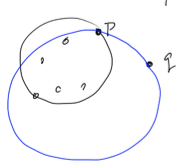
\includegraphics{images/smallest_disc.png}
                    \caption{Smallest Disc}
                    \label{fig:smallest_disc}
                \end{figure}
                Using this principle leads to an expected\footnote{TODO: Why isn't this guaranteed?} runtime of $O(n)$.
            % section randomized_incremental_disc_fitting (end)
        % chapter linear_programming (end)
        \chapter{Randomized Algorithms for Satisfiability (\textsc{sat})} % (fold)
        \label{cha:randomized_algorithms_for_satisfiability_}
            Generally, satisfiability is the question that asks that given a boolean formula with $n$ variables and $m$ clauses when expressed in CNF, can we assign \textsc{truth} or \textsc{false} values to \uline{satisfy} the formula.
            In the example below with $E$, assigning $x_1$ and $x_2$ satisfies the formula:
            \begin{align*}
                E &= (x_1 \lor x_2 \lor x_3) \land (x_1 \lor \lnot x_2) \land (\lnot x_1 \lor \lnot x_2 \lor \lnot x_3) \land (x_2 \lor \lnot x_3) \\
                x_1 &= \text{\textsc{true}} \\
                x_3 &= \text{\textsc{false}}
            \end{align*}
            The \textsc{3-sat} algorithm is an \np-variant where all clauses have $3$ distinct literals.
            The \textsc{2-sat} algorithm can be solved in polynomial time (in fact, $O(n)$ time).

            We can apply this to everything, as it helps with quantified boolean formulae.
            \textsc{sat} is a case of one (implicit) $\exists$ quantifier.

            \section{Techniques for \textsc{sat}} % (fold)
            \label{sec:techniques_for_sat}
                There are heuristics that help us ``resolve'' different clauses.
                In fact, we can solve 3-SAT (in a non-obvious way) in $O(1.5^n)$ time using deterministic algorithms instead of the obvious $O(2^n \text{poly}(n, m))$.

                Using randomized algorithms, we're going to get better than $O(1.5^n)$ for 3-SAT\footnote{By concentrating on 2-SAT then broadening our scope to 3-SAT.}.

                We are unlikely to get randomized polynomial time algorithms, since this implies randomized poly-time for all problems in \np. (eek)
            % section techniques_for_sat (end)
            \section{Randomized SAT Solving} % (fold)
            \label{sec:randomized_sat_solving}
                The idea is that we're going to be given an input $E$ in CNF, then we're going to ``hill climb'' to better values.
                This algorithm is called Papadimitrion's algorithm (`91).
                \begin{verbatim}
    randomly assign T/F assignment A
    for i = 1...t:
        if A satisfies E return YES
        pick a random unsatisfied clause C
        randomly pick a literal x in C
        flip x's value
    return NO (maybe)
                \end{verbatim}
                We want to choose $t$ and determine the error probability.

                Errors occur when $E$ is satisfiable and we return \textsc{no}.

                Suppose $A^*$ is a truth value assignment that satisfies $E$.
                For $i$ as the number of variables with same value in $A$ and $A^*$, we can say that if $i$ reaches $n$, then $A = A^*$ and the algorithm outputs \textsc{YES}.

                When we re-assign the value of the variable, we know that $i$ goes up or down by $1$.

                \subsection{Randomized Walk on a Line} % (fold)
                \label{sub:randomized_walk_on_a_line}
                    To do this analysis, we need to know about random walks on lines.

                    Start at a randomly chosen $i$, each step moves right (\verb|i++|) with probability $\frac{1}{2}$ and left (\verb|i--|) with probability $\frac{1}{2}$.
                    When $i=0$, we always go right.
                    When $i=n$, we terminate.

                    The question can now be phrased as:
                    What are the expected number of steps to get to $n$?

                    Alternatively, we can analyze this as a Markov chain, or a finite automaton with probabilistic state movements.

                    We're now looking for the expected number of steps to get from $i$ to $n$ - denoted $t_i$.
                    \begin{align*}
                        t_n &= 0 \\
                        t_0 &= 1 + t_1 \\
                        t_i &= 1 + t_{i-1} \frac{1}{2} + t_{i+1} \frac{1}{2}
                    \end{align*}
                    This is awkward for induction, but if we rearrange it, it's pretty smooth:
                    \begin{align*}
                        t_i + t_{i+1} &= 2 (t_{i-1} - t_{i}) \\
                        d_i &= t_i + t_{i+1} \\
                        d_0 &= t_0 - t_1 \\
                        &= 1 \\
                        d_i &= 2 + d_{i - 1} \\
                        &= 1 + 2i
                    \end{align*}
                    If we substitute this for $t_i$, we get:
                    \begin{align*}
                        t_i &= d_i + t_{i + 1} \\
                        t_n &= 0 \\
                        t_i &= \sum_{j=1}^{n-1} d_J \\
                        &= \sum_{j=1}^{n-1} (1 + 2j) \\
                        &= n-1 + \sum_{j=1}^{n-1} j \\
                        &= (n - i) + n(n-1) - i (i - 1) \\
                        &= n^2 - i^2
                    \end{align*}
                    The maximum is $t_0 = n^2$, and $t_i \le n^2$.
                % subsection randomized_walk_on_a_line (end)
                \subsection{Finding Error in our Approximation} % (fold)
                \label{sub:finding_error_in_our_approximation}
                    For Papadimitrion's solution to 2-\textsc{sat}, we can model the number of steps as a random walk on a line.
                    In this representation, we say $t_i$ is a state where $i$ variables are ``set correctly'', and assume the worst case scenario of only one assignment being correct.

                    In a clause $C = (\alpha \lor \beta)$ being modified was not satisfied, then one of $\alpha$ or $\beta$ must be true in the optimal solution.
                    If only one needs to be inverted, we pick the correct one $\frac{1}{2}$ the time.
                    If both need to be inverted, we pick the correct one every time.
                    So we can say that the probability that $i$ increases is $\ge \frac{1}{2}$.

                    By strategically picking the value of $t$, we can easily determine the expected number of repeats.
                    Using Markov's inequality (which can be found in Section~\ref{sec:markov_s_inequality}):

                    Supposing $X \ge 0$ and $E(X) = \mu$, then $\Pr\{ X \ge c \mu\} \le \frac{1}{c}$ for a constant $c$.
                    In our case, $\mu = n^2$, so we choose $c = 2$.
                    \begin{align*}
                        \Pr \{ \text{\# steps} > 2n^2 \} &< \frac{1}{2}
                    \end{align*}
                    So set $t = 2n^2$, then $\Pr\{\text{error}\} < \frac{1}{2}$.

                    From this we know that the runtime is not $O(n^2)$, but it actually is $O(n^2 \cdot poly(n, m))$ time.
                % subsection finding_error_in_our_approximation (end)
                \subsection{Papadimitrion's Algorithm in Higher Dimensions} % (fold)
                \label{sub:papadimitrion_s_algorithm_in_higher_dimensions}
                    For a given clause $C = (\alpha \lor \beta \lor \gamma)$, if $A$ does not satisfy $C$, but $A^*$ does with $\alpha = T$.
                    \begin{align*}
                        \Pr(\text{Algorithm flips $\alpha$}) &= \frac{1}{3} \\
                        \Pr(\text{$i$ increases}) &\ge \frac{1}{3}
                    \end{align*}
                    So we analyze a random walk on a line:
                    \begin{align*}
                        \Pr(\text{i goes to $i+1$}) &= \frac{1}{3} \\
                        \Pr(\text{i goes to $i-1$}) &= \frac{1}{3}
                    \end{align*}
                    Using Markov's inequality as before, we are expected to take $\approx 2^n$ steps to get to $n$, the final value\footnote{Analysis omitted from course slides.}.
                % subsection papadimitrion_s_algorithm_in_higher_dimensions (end)
                \subsection{Sch\"{o}ning's Algorithm} % (fold)
                \label{sub:sch_ning_s_algorithm}
                    Sch\"{o}ning (`99) gives two improvements to the algorithm:
                    \begin{itemize}
                        \item Start with a random assignment $A$
                        \item An increasing number of trials is not helpful if we've taken many steps without reaching $A^*$.
                        We're probably stuck near or at $0$, so lets pick a ``new'' random $A$.
                    \end{itemize}
                    \begin{verbatim}
schoning(E):
    for i = 1...s:
        randomly pick A
        repeat t = 1...3n:
            if A satisfies E output YES
            else
                pick unsatisfied clause C
                randomly flip a variable in C
    output NO-MAYBE
                    \end{verbatim}
                    In the inner loop, the probability of error is $\Pr(\text{error}) \lesssim 1 - \left( \frac{3}{4} \right)^n$.

                    When we set $S = c \left( \frac{3}{4} \right)^n$, the probability of error $\Pr(\text{error}) \lesssim (1 - \left( \frac{3}{4} \right)^n)^{c \left(\frac{4}{3} \right)^n}$.

                    From calculus, we know that $\left( 1 - \frac{1}{a} \right)^a \le \frac{1}{e}$, so the probability of error is $\Pr(\text{error}) \lesssim \frac{1}{e^c}$.

                    The bottom line is that we get $\Pr(\text{error}) \le \frac{1}{2}$, with runtime $O\left( \left(\frac{4}{3} \right)^n n \right)$.
                    While this is exponential, it does beat the best known non-randomized algorithm that we know.
                % subsection sch_ning_s_algorithm (end)
            % section randomized_sat_solving (end)
        % chapter randomized_algorithms_for_satisfiability_ (end)
        \chapter{Minimum Spanning Trees} % (fold)
        \label{cha:minimum_spanning_trees}
            The problem \textsc{mst} can be expressed as follows:
            \begin{quotation}
                Given an undirected graph $G = (V, E)$ with edge weights $w : E \to \mathbf{R}^+$, find a minimum-weight spanning tree.
            \end{quotation}
            In other words, find the tree on the graph that reaches all vertexes such that has the minimal total of edge weight in the tree.

            Let's assume that edge weights are distinct\footnote{If they aren't, we only need to break ties consistently.}.

            We can generate this problem to a spanning forest of disconnected graph\footnote{I have no clue what this means.} %TODO: What does this mean?

            There are two basic rules:
            \begin{description}
                \item[Inclusion Rule] The inclusion rule dictates that for a given vertex $v$, if $v$'s minimum weight incident edge\footnote{An incident edge to $v$ is an edge between $v$ and another vertex.} is $e = vu$, then $vu \in \textsc{mst}(G)$.
                    Since we know this, we can \uline{contract} the vertexes $v$ and $u$ into each other creating a vertex $v'$, and continue the process with a smaller graph.
                    For every vertex $r$ which has an edge to both $v$ and $u$, we just add the smaller of the two edges to $v'$.
                \item[Exclusion Rule] The exclusion rule dictates that for a given cycle $C$ with maximum weight edge $e$, then $e \not \in \textsc{mst}(G)$.
                    We may delete $e$ and continue.
            \end{description}
            While basically all \textsc{mst} algorithms work under these rules, we can't get the MST without contraction.

            In this analysis, $n$ is the number of vertexes, and $m$ is the number of edges.

            \section{Kruskal's Algorithm (`56)} % (fold)
            \label{sec:kruskal_s_algorithm_}
                Kruskal's Algorithm uses the inclusion rule.
                \begin{verbatim}
    mst(G)
        repeat:
            e = (u, v) = minimumWeightEdge(G)
            T += uv
            contract(G, e)
        end
                \end{verbatim}
                By sorting edges by weight, then using union-find to find the new vertexes connected to edges after contraction, this algorithm takes $O(m \log n)$ time.
            % section kruskal_s_algorithm_ (end)
            \section{Prim's Algorithm (`57)} % (fold)
            \label{sec:prim_s_algorithm_57}
                \begin{verbatim}
    mst(G):
        S = randomVertexFrom(G.V)
        repeat:
            e = minimumWeightEdgeFrom(S)
            T += e
            contract(G, e)
            S.put(e.from)
            S.put(e.to)
                \end{verbatim}
                Implementing with a heap takes $O(m \log n)$ time.
                Implementing with a Fibonacci Heap takes $O(n \log n + m)$ time, which is linear when $m > n \log n$.
            % section prim_s_algorithm_57 (end)

            \section{Bor\r{u}vka's Algorithm (`26)} % (fold)
            \label{sec:borukva_s_algorithm_26}
                The idea is that we want to apply the inclusion rule to all vertexes at once.
                We'll actually just apply it until every vertex is a contracted one, and the resultant number of vertexes is $\le \frac{n}{2}$.
                \subsection{Bor\r{u}vka Step} % (fold)
                \label{sub:baruvka_step}
                    The is that we want to ensure every vertex is part of at least one merge.
                    \begin{verbatim}
    baruvka(G):
        unmark all vertexes
        for each v in V:
            if v is unmarked:
                find minimum weight edge e=vu
                add e to T, contract v to u
                mark u
        return T
                    \end{verbatim}
                    For each vertex $v$, the Bor\r{u}vka Step checks $v$'s minimum weight edge, and contracts $v \to u$, which takes $O(\text{deg}(v))$ time.
                    Thus, the entire step takes:
                    \begin{align*}
                        O\left(\sum_v \text{deg}(v) \right) &= O(m)
                    \end{align*}
                    The step reduces the graph to $\le \frac{n}{2}$ vertexes.
                % subsection baruvka_step (end)
                \subsection{Bor\r{u}vka's Algorithm} % (fold)
                \label{sub:baruvka_s_algorithm}
                    The idea is to repeat the Bor\r{u}vka Step until only one vertex is left.

                    Since there are going to be $O(\log n)$ reductions, the total time is $O(m \log n)$.
                    This isn't as fast in practice as Prim, but it's much simpler to implement.
                % subsection baruvka_s_algorithm (end)
            % section borukva_s_algorithm_26 (end)
            \section{History of MST Algorithms} % (fold)
            \label{sec:history_of_mst_algorithms}
                \begin{itemize}
                    \item In `75, Yao, Cheriton, and Tarjan found a $O(m \log \log n)$ algorithm.
                    \item In `85, Fredman and Tarjan found a $O(m \log^* n)$ algorithm.
                    \item In `87, Chazelle found an $O(m \alpha(n))$ algorithm.
                \end{itemize}
                \open: Is there a linear time ($O(n + m)$) algorithm?
            % section history_of_mst_algorithms (end)
            \section{Karger's Algorithm (`93)} % (fold)
            \label{sec:karger_s_algorithm_}
                Karger gave a Las-Vegas MST algorithm with linear expected run time.
                The idea of his algorithm is to use random sampling, the exclusion rule, and recursion.

                We want the algorithm $\textsc{mst}(E)$ to return the \textsc{mst} of each connected component of $G=(V, E)$.

                \begin{verbatim}
    MST(E):
        take a random subset R <= E of size |R| = r // chosen later: r=2n
        T = MST(R)
        for each edge uv in E, do:
            if uv is not in T and uv is heavier than all edges in the uv path in T:
                classify uv as heavy
            else:
                classify uv as light and replace uv with e in T
        E = E - heavy edges
        return MST(E)
                \end{verbatim}
                This is correct by the exclusion rule.
                If we added a new edge $e = uv$ to the sample $R$:
                \begin{itemize}
                    \item If $e$ is heavy, $T$ does not change.
                    \item If $e$ is light, we would've updated $T$ to use $uv$.
                \end{itemize}
                Additionally $T$ is the \textsc{mst} of the entire graph iff all edges not in $T$ are heavy.

                We can classify edges and verify if $T$ is a \textsc{mst} of the entire graph in $O(m)$ time\footnote{In class, she alluded that this is complicated, and didn't go any further. At the bottom of her notes though, there is a link to \href{https://www.cs.cmu.edu/afs/cs.cmu.edu/academic/class/15750-s01/www/notes/lect0208}{A CMU grad course's (link)} explanation of the matter.}.

                \subsection{Sampling Lemma} % (fold)
                \label{sub:sampling_lemma}
                    We propose that the number of light edges $E(\text{\# light edges}) \le \frac{mn}{r}$.
                    Since there are $m$ edges, this is enough to show that $\Pr(\text{e is light}) \le\frac{n}{r}$.

                    We can prove this by working backwards:
                    Consider $R' = R \cup \{e\}$, where $e$ is a random element of $R'$.
                    By the notes above, $e$ is light with respect to $R$ if and only if $e$ is in the $\textsc{mst}(R')$ (which has $\le n-1$ edges).
                    So $\Pr(\text{$e$ is light}) \le \frac{n-1}{|R'|} < \frac{n}{r}$.
                % subsection sampling_lemma (end)
                \subsection{Analysis of Expected Runtime} % (fold)
                \label{sub:analysis_of_expected_runtime}
                    We have the following recursion:
                    \begin{align*}
                        T(m, n) &= \text{recursive call on $R$} + \text{time to classify} + \text{recursive call to find the MST of $E$-heavy} \\
                        T(m, n) &= T(r, n) + O(m + n) + T\left(\frac{mn}{r}, n\right)
                    \end{align*}
                    With $r = 2n$, this becomes:
                    \begin{align*}
                        T(m, n) &= T(2n, n) + O(m + n) + T\left(\frac{mn}{2n}, n\right) \\
                        T(m, n) &= T(2n, n) + T\left(\frac{m}{2}, n\right) + O(m + n)
                    \end{align*}

                    The final idea, (attributed to Karger, Klein, and Tarjan in `94) is on each recursive call to do 3 Bor\r{u}vka steps first.
                    This reduces $\text{\# vertexes} \le \frac{n}{8}$ with $O(n + m)$ work.
                    For some constant $d$, we have:
                    \begin{align*}
                        T(m, n) \le T\left(\frac{n}{4}, \frac{n}{8}\right) + T\left(\frac{m}{2}, \frac{n}{8}\right) + d(m+n)
                    \end{align*}
                    Proving that $T(m, n) \le c(m + n)$ for some constant $c$ is sufficient to prove $T(m, n) \in O(n + m)$.
                    We implicitly assume that the base case has been proven, and prove the inductive step:
                    \begin{align*}
                        T(m, n) &\le c\left(\frac{n}{4} + \frac{n}{8}\right) + c\left(\frac{m}{2} + \frac{n}{8}\right) + d\left(m + n\right) \\
                                &= \left(\frac{c}{2} + d\right) n + \left(\frac{c}{2} + d \right) m \\
                                &\le c(n+m) \text{ as long as $\frac{c}{2} + d \le c$}
                    \end{align*}
                    So the expected runtime is $O(m+n)$.
                % subsection analysis_of_expected_runtime (end)
            % section karger_s_algorithm_ (end)
        % chapter minimum_spanning_trees (end)
    % part data_ _structures_ (end)
    \part{Approximating Hard Things} % (fold)
    \label{prt:approximating_ _hard_ _things_}
        \chapter{Approximation Algorithms} % (fold)
        \label{cha:approximation_algorithms}
            Recall $\p \stackrel{?}{=} \np$.

            We have a set $\p \subseteq \np$, and another set $\npcomplete \subseteq \np$, where \npcomplete are the hardest problems in \np.
            There are a few problems in \np that are not in \p and not known to be in \npcomplete (factoring, graph isomorphism, etc).

            It is \open  if there exist poly-time correct algorithms to solve \npcomplete problems.

            Ladner proved that:
            \begin{quotation}
                If $\p \not = \np$, then there are infinitely many problems in the space between \p and \npcomplete.
            \end{quotation}

            It seems like we must either give up correctness, or speed.

            And thus, approximation algorithms are born.
            For optimization problems, these algorithms guarantee that their result is \textit{close to} the optimal solution.

            \section{Concerning Approximation Algorithms} % (fold)
            \label{sec:concerning_approximation_algorithms}
                An \uline{approximation} algorithm finds in polynomial-time a solution that is close to the optimal, either in terms of ratio or in constant difference.

                \subsubsection{Edge-Coloring in a Graph} % (fold)
                \label{ssub:edge_coloring_in_a_graph}
                    Given a graph $G$, color the edges such that if two edges are incident\footnote{Two edges are incident if they share a vertex.}, they have different colors.

                    A variant of this problem is \npcomplete:
                    \begin{quotation}
                        Given $G$ and $k \in \mathbf{N}$, can you edge color $G$ with $k$ colors?
                    \end{quotation}

                    Vizing's Theorem states that for the maximum degree across all vertexes in a graph $\Delta$, $\Delta \le \text{minimum number of colors} \le \Delta +1 $.

                    Furthermore, there exists a polynomial-time algorithm to color any graph with $\Delta+1$ colors.

                    Since the algorithm exists, we can approximate within $+1$ of the \opt solution.

                    This type of approximation (constant additive) is rare, since we usually get a good ratio of \appr to \opt.
                % subsubsection edge_coloring_in_a_graph (end)
                \subsubsection{Vertex Cover} % (fold)
                \label{ssub:vertex_cover}
                    Given a graph $G = (V, E)$, find a minimum-size \uline{vertex cover}\index{Vertex Cover} - a set $U \subseteq V$ such that every edge has at least one endpoint in $U$.

                    We can use this kind of algorithm to monitor all links in a network.

                    The decision version of Vertex-Cover is \npcomplete.
                    Where Independent set is the question to find the maximum set of vertexes where no two are joined by an edge, there is a reduction this way:
                    \begin{align*}
                        \textsc{3sat} \le_p \text{independent set} \le_p \text{vertex cover}
                    \end{align*}
                    The argument for reduction between vertex cover and independent set is that $U \subseteq V$ is a minimum vertex cover if and only if $V - U$ is a maximum independent set.

                    The existence of an approximation algorithm for vertex cover that's good within an additive constant (as for edge coloring) implies \p = \np.
                % subsubsection vertex_cover (end)
            % section concerning_approximation_algorithms (end)
            \section{Greedy Algorithm for Max Vertex Cover} % (fold)
            \label{sec:greedy_algorithm_for_max_vertex_cover}
                \begin{lstlisting}
maxCover(V):
    C = [];
    while true:
        if no edges remain: break;
        C.append(vertex of max degree)
        remove covered edges
                \end{lstlisting}
                We will show that $|C| \le O(\log n) |\opt|$.

                Exercise for reader (not in notes):
                Show that the greedy algorithm can give $\frac{|C|}{|\opt|} \in \Omega (\log n)$.
            % section greedy_algorithm_for_max_vertex_cover (end)
            \section{Set Cover Problem} % (fold)
            \label{sec:set_cover_problem}
                The max vertex problem is a subset of the Set Cover problem.

                Given a collection of sets $S_1, S_2, \ldots, S_k$ where $S_i \subseteq [1, n]$.
                Find a minimum sized set $C \subseteq [1, n]$ such that for all $i \in [1, n]$, $i \in S_j$ for some $j \in C$.

                In the real world, this works as follows:
                \begin{quote}
                    Where sets $S_i$ are a type of pizza, and set elements $e$ are individual people.
                    An element $e \in S_i$ means that the person eats that type of pizza.
                    We want to find the minimum number of pizza types to feed all people.
                \end{quote}

                \subsection{Vertex vs Set Cover} % (fold)
                \label{sub:vertex_vs_set_cover}
                    We can show that vertex cover is a special case of Set Cover:
                    Elements $e$ of our sets are edges in the graph,
                    and sets correspond to vertexes in our graph.

                    Since every element in our vertex cover is in exactly two of our sets, a
                    A Set Cover that every element is in exactly two of our sets allows us to transform our Set Cover problem into a vertex cover.
                % subsection vertex_vs_set_cover (end)
                \subsection{Greedy Approximation Algorithm for Set Cover} % (fold)
                \label{sub:greedy_approximation_algorithm_for_set_cover}
                    The idea is to iteratively choose the set that has the most yet uncovered elements.
                    \begin{lstlisting}
setCover(S[] s):
    C = []
    while there are uncovered elements:
        S[i] = a set that covers the max number of uncovered elements
        C.append(i)
                    \end{lstlisting}
                    We claim that $|C| = \appr \le O(\log n) \opt$, where \opt is the minimum number of sets to cover all elements.

                    % TODO: Build an external reference to Vazirani.
                    This proof is taken from Vazirani's book\footnote{This seems to be the only reference to Vazirani in her notes, but she mentions in class that he visited UWaterloo a while ago and showed her a misprint in the subtitle of an old version of his book.}, which is a simpler proof than the one presented in CLRS.

                    We distribute the cost (1) of choosing a set $S_i$ over the newly covered elements.
                    Let $c(e)$ represent the cost of adding element $e$.

                    We define $S$ as the maximum size set, since it is the first one chosen.
                    For a defined element $e \in S$, we define $c(e) = \frac{1}{|S|}$.
                    We know that $|S| > $ the average number of elements per set in the \opt solution.
                    We also know that the average number of elements $n$ per set in the \opt solution is $\ge \frac{n}{\opt}$.
                    This implies that for the first set we have:
                    \begin{align*}
                        c(e) &\le \frac{\opt}{n}
                    \end{align*}

                    More generally, let the ordering $e_1, e_2, \ldots, e_i, \ldots e_n$ be an ordering of elements as they are covered (we expect many ties).

                    We define that the number elements newly covered by $S'$ as $k$.
                    For a given $e_i \in S'$, we know that the number of elements uncovered prior to $S'$ being chosen must be $\ge n - i + 1$.

                    Since the set picked is the one with the maximal $k$, we know that it must be $\ge \textsc{avg}$ on the range $j \ge i$ covered by \opt.
                    We know that $\textsc{avg} \ge \frac{n-i+1}{\opt}$, since any lower would mean that there are more than \opt sets chosen in the \opt solution.
                    Thus, $k \ge \frac{n-i+1}{\opt}$, which implies that $c(e_i) \le \frac{\opt}{n-i+1}$.

                    \begin{align*}
                        \text{number of sets chosen by greedy} &= \sum_{i=1}^n c(e_i) \\
                        &\in O(\log n) \opt
                    \end{align*}
                    Thus, the number of sets chosen by the greedy is within a factor of $O(\log n) \opt$.
                % subsection greedy_approximation_algorithm_for_set_cover (end)
            % section set_cover_problem (end)
        % chapter approximation_algorithms (end)
        \chapter{Linear Programs and Randomization} % (fold)
        \label{cha:linear_programs_and_randomization}
            \section{Vertex Cover} % (fold)
            \label{sec:vertex_cover}
                Please recall the definition of the vertex cover problem on page \pageref{ssub:vertex_cover}, and the approximation within $O(\log n) \opt$ presented on page \pageref{sec:greedy_algorithm_for_max_vertex_cover}.
                \subsection{Constant-Factor Approximation for Vertex Cover} % (fold)
                \label{sub:constant_factor_approximation_for_vertex_cover}
                    There's a ``stupid'' approximation algorithm for vertex cover that's better than the greedy algorithm.
                    \begin{lstlisting}
vertex_cover(E, V):
    C = {}
    while E != {}:
        (u, v) = E.remove_random()
        e = {u, v}
        C.append(e)
        E.remove_connected_to([u, v])
    return C
                    \end{lstlisting}
                    Since we pick the set of edges is a matching\footnote{A matching $M$ is a set of edges such that no two share a common vertex.}.
                    Where $M$ is the set of edges we pick, we know that $|C| = 2|M|$.
                    We also know that $|M| \le \opt$, since every matching edge needs its own vertex in the \opt vertex cover.

                    Thus, our ``stupid'' greedy algorithm has $|C| = 2|M| \le 2 \opt$, and thus gives us an approximation factor of 2.
                    \subsubsection{Best Approximation Factor Known for Vertex Cover} % (fold)
                    \label{ssub:best_approximation_factor_known_for_vertex_cover}
                        The best approximation factor known for the Vertex Cover problem is 2.
                    % subsubsection best_approximation_factor_known_for_vertex_cover (end)
                % subsection constant_factor_approximation_for_vertex_cover (end)
                \subsubsection{Weighted Vertex Cover} % (fold)
                \label{ssub:weighted_vertex_cover}
                    \begin{quotation}
                        Given weights on vertices $w : V \to \mathbf{R}^+$, find the vertex cover $C$ of minimum weight $\sum_{v \in C} w(v)$.
                    \end{quotation}
                    In fact, we can express this as an integer linear program.

                    Create a variable $x(v)$ for each $v \in V$.
                    \begin{align*}
                        x(v) = \left\{
                            \begin{array}{lr}
                                1 & : v \in C \\
                                0 & : v \notin C
                            \end{array}
                        \right.
                    \end{align*}

                    Now we're trying to find the solution to the following linear program:
                    \begin{align*}
                        \min \sum_{v \in V} w(v) x(v)
                    \end{align*}
                    Given the constraints that $\forall e \in E : e = (u, v) : x(u) + x(v) \ge 1$, and bounding the values of $x()$ to be $x(v) \in \{0, 1\}$.

                    The solutions to this integer linear program are exactly minimum-weight vertex covers.
                    While Integer Linear Programs (\textsc{ILP}) are \npcomplete\footnote{There is no proof given, and Chapter~\ref{cha:linear_programming} doesn't deal with this type of problem.}, relaxing the constraints to be non-integer Linear Program (\textsc{LP}) allows us to use the simplex method (Refex to Subsection~\ref{sub:simplex_method}).
                    To use simplex, we can relax $x(v) \in \{0, 1\}$ to $x(v) \in [0, 1]$.

                    Suppose that $\bar{x}$ is an optional solution to the linear program.
                    Let $C_{\textsc{LP}} = \{ v \in V : \bar{x}(v) \ge \frac{1}{2} \}$.
                    Our linear program guarantees that $\bar{x}(u) + \bar{x}(v) \ge 1$, so at least one of $u, v$ has $\bar{x}(-) \ge \frac{1}{2}$, and that vertex is definitely in $C_{\textsc{LP}}$.
                    Then $C_{\textsc{LP}}$ is a vertex cover.

                    Starting with the premise that $\opt = \opt \text{ to } \textsc{ILP} \ge \opt \text{ to } \textsc{LP}$, since the \textsc{lp} allows more solutions, so the \opt decreases.
                    Given that $\bar{x}(-)$ is the \opt solution to the \textsc{LP}, we have:
                    \begin{align*}
                        \opt &= \sum w(v) \bar{x}(v) \\
                        &\ge \sum_{v \in V : \bar{x}(v) \ge 0.5} w(v) \bar{x}(v) \\
                        &\ge \sum_{v \in V : \bar{x}(v) \ge 0.5} w(v) \frac{1}{2} \\
                        &= \frac{1}{2} \sum_{v \in V : \bar{x}(v) \ge 0.5} w(v) \\
                        &= \frac{1}{2} w(C_{\textsc{LP}})
                    \end{align*}
                    So $\opt \ge \frac{1}{2} w(C_{\textsc{LP}})$ or $w(C_{\textsc{LP}}) \le 2 \opt$.

                % subsubsection weighted_vertex_cover (end)
            % section vertex_cover (end)
            \section{Set Cover Problem} % (fold)
            \label{sec:set_cover_problem}
                \begin{quotation}
                    Given a collection of sets $S_1, S_2, \ldots S_k$, where $S_i \subseteq \{1, \ldots, n \}$, find a minimum size set of sets such that every element is covered.
                \end{quotation}
                In other words, find $C \subseteq \{ 1, \ldots, k\}$ such that $\forall i \in \{1, \ldots, n\}$, $i \in S_j$ for some $j \in C$.

                For a Set Cover, the greedy algorithm gives $\le O(\log n) \opt$ (refer to Subsection~\ref{sub:greedy_approximation_algorithm_for_set_cover}).

                There's something that's marginally better.
                Define $f$ as the maximum number of sets any single element $e$ is contained in.
                For vertex cover, the elements are edges, and the sets are edges incident to a vertex $v$.
                $f$ for vertex cover is 2, so it is a special case of Set Cover.

                There is a polynomial time approximation algorithm using linear programming and duality for Set Cover that gives a solution of $\le f \opt$, which is an approximation factor $f$.

                Depending on the difference between $\log n$ and $f$, one may be factor.

                % TODO: link to the ``later'' I refer to
                Later, we will prove that Set Cover has no constant factor approximation in polynomial time unless $\p = \np$.

                \subsubsection{Approximation For Minimization and Maximization Problems} % (fold)
                \label{ssub:approximation_for_minimization_and_maximization_problems}
                    A $\rho$-approximization algorithm for a minimization problem guarantees that $A(I) \le \rho \opt(I)$, so $\rho \ge 1$.

                    A $\rho$-approximization algorithm for a maximization problem guarantees that $A(I) \ge \rho \opt(I)$, so $\rho \le 1$.

                    Some texts use $\frac{1}{\rho}$ for maximization problems.
                    CLRS doesn't do max, and Vazirani uses the convention here.
                % subsubsection approximation_for_minimization_and_maximization_problems (end)
                \subsubsection{Max-Cut Problem} % (fold)
                \label{ssub:max_cut_problem}
                    The Max Cut problem is a sub-type of the Set Cover problem.
                    \begin{quotation}
                        Given a graph $G = (V, E)$, partition $V$ into $S$, $V - S$ to maximize the number of edges with one end in $S$ and another end in $S$.
                    \end{quotation}
                    We define $c(S)$ as the size of cut\footnote{That is, the number of edges cut.} for $S$, $V - S$.

                    Without proof, the (decision version of the) Max-Cut problem is \npcomplete, but the minimum cut can be found in polynomial time.

                    An approximation for Max Cut is as follows:
                    \begin{lstlisting}
max_cut(G):
    S = V.any_subset()
    while vertexes can be moved to increse c(S):
        move a vertex to increase c(S)
                    \end{lstlisting}
                    Given that we can increase $c(S)$ at most $m$ times\footnote{As usual, $m$ is the number of edges.}, we must have a polynomial time algorithm.

                    Define the number of edges inside $S$ as $e(s)$, and the number of edges from $v$ to $S$ as $d_S(v)$, and the number of edges from $v$ to $V-S$ as $d_{V-S}(v)$.
                    At the end of the algorithm, $\forall v \in S$, $d_S(v) \le d_{V-S}(v)$, otherwise we would move it.
                    \begin{align*}
                        \sum_{v \in S} d_{V - S}(v) &\ge \sum_{v \in S} d_S(v) \\
                        \implies 2e(S) &\le c(S) \\
                    \end{align*}
                    Similarly $\forall v \in V-S$:
                    Thus:
                    \begin{align*}
                        d_{V-S}(v) &\le d_{S}(v) \\
                        \sum_{v \in V-S} d_{V-S}(v) &\le \sum_{v \in V-S} d_S(v) \\
                        \implies 2e(V-S) &\le c(S)
                    \end{align*}

                    Since $m = e(S) + e(V-S) + c(S)$, we can say:
                    \begin{align*}
                        m &= e(S) + e(V-S) + c(S) \\
                        2m &= 2e(S) + 2e(V-S) + 2c(S) \\
                        &\le c(S) + c(S) + 2c(S) \\
                        &= 4c(S)
                    \end{align*}
                    Thus $m \le 2 c(S)$, which means we have an approximation factor of $\frac{1}{2}$.
                % subsubsection max_cut_problem (end)
                \subsubsection{Random Algorithm for Max Cut Problem} % (fold)
                \label{ssub:random_algorithm_for_max_cut_problem}
                    \begin{lstlisting}
max_cut(G):
    pick S at random
                    \end{lstlisting}
                    We can do this analysis:
                    \begin{align*}
                        E[c(S)] &= E\left[ \sum_{e \in E} \sigma(e) \right] \\
                        \sigma(e) &=
                            \left\{
                                \begin{array}{lr}
                                    1 :& \text{ if $e$ in cut }\\
                                    0 :& \text{ otherwise }
                                \end{array}
                            \right. \\
                        E[c(S)] &= \sum_{e \in E} E[\sigma(e)] \\
                        &= \sum_{e \in E} \frac{1}{2} \\
                        &= \frac{m}{2}
                    \end{align*}
                    By doing this repeatedly, we can get a $O(n)$-time algorithm with a $\frac{1}{2}$ approximation factor.
                % subsubsection random_algorithm_for_max_cut_problem (end)
                \subsubsection{State of the Art in Max Cut} % (fold)
                \label{ssub:state_of_the_art_in_max_cut}
                    The best known approximation factor for Max Cut is $0.878$ (unattributed).
                % subsubsection state_of_the_art_in_max_cut (end)
            % section set_cover_problem (end)
        % chapter linear_programs_and_randomization (end)
        \chapter{Max SAT} % (fold)
        \label{cha:max_sat}
            \begin{quotation}
                Given a set of $m$ clauses in \textsc{CNF} in $n$ boolean variables $X = \{x_1, \ldots, x_n\}$, find a boolean assignment to variables to make a maximum number of clauses true.
            \end{quotation}
            The decision version of this problem is \npcomplete, since it's just the usual \textsc{sat} problem.
            For clauses of size $\le 2$, it is still \npcomplete.
            For problems with clauses are size 2, deciding if \uline{all} can be satisfied is in \p\footnote{To prove that it is \npcomplete, we only need to reduce 3-\textsc{sat} to Max 2-\textsc{sat}, just turn $(x \lor y \lor z)$ into about 10 2-\textsc{sat} clauses such that $(x \lor y \lor z)$ is satisfied if about 7 of the 2-\textsc{sat} clauses are satisfied.}.

            \section{Algorithm for Max-\textsc{SAT}} % (fold)
            \label{sec:algorithm_for_max_sat}
                The algorithm is to pick the truth assignment at random.

                We know that for any clause $c$ containing $t$ different variables, we want to determine the probability that $c$ is satisfied:
                \begin{align*}
                    \textsc{Pr}(\text{$c$ is satisfied}) &= 1 - \textsc{Pr}{\text{$c$ is not satisfied}} \\
                    &= 1 - \frac{1}{2^t} \\
                    &\ge (1 - \frac{1}{2}) \\
                    &= \frac{1}{2}
                \end{align*}
                Thus the expected number of clauses satisfied is $\ge \frac{1}{2} m$.

                We know that $\opt \le m$, so the expected \appr factor is $\frac{1}{2}$.
            % section algorithm_for_max_sat (end)
            \section{Facts about the Max-\textsc{SAT} problem} % (fold)
            \label{sec:facts_about_the_max_sat_problem}
                By the probabilistic method\footnote{Not explained in class, but apparently there are many powerful consequences.}, there always exists a truth value assignment that satisfies at least half the clauses.

                The proof is essentially that since the expected value of a random variable  is $\alpha$, then there is at least one value for the variable that has value $\ge \alpha$.
            % section facts_about_the_max_sat_problem (end)
            \section{Improved Algorithm for Max-\textsc{Sat}} % (fold)
            \label{sec:improved_approximation_algorithm_for_the_max_sat}
                By formulating this as an ILP problem, we can solve this using a LP relaxation (Similar to the Weighted Vertex Cover solution on Page \pageref{ssub:weighted_vertex_cover}) and ``randomized rounding'' techniques.

                Make variables $x_i$, $i \in [1, n]$ for each boolean variable $a_i$, and $y_i$, $i \in [1, m]$ for each clause.

                We want to maximize $\sum_i y_i$.

                We have one constraint per clause:
                \begin{align*}
                    c_1 = (\bar{a_1} \lor a_2) &\to y_1 \le (1 - x_1) + x_2
                \end{align*}
                And we have the LP relaxation constraints:
                \begin{align*}
                    0 \le &x_i \le 1 : i \in [1, n] \\
                    0 \le &y_i \le 1 : i \in [1, m]
                \end{align*}

                Using the \p LP approximation, we solve for $x$'s.

                Then, we set our truth values $A = \{ a_0, \ldots, a_n\}$ as follows:
                \begin{align*}
                    a_i &=
                        \left\{
                            \begin{array}{lr}
                                1 :& \text{ with probability $x_i$ }\\
                                0 :& \text{ otherwise }
                            \end{array}
                        \right.
                \end{align*}

                \subsubsection{Analysis of Randomized Max 2-\textsc{sat}} % (fold)
                \label{ssub:analysis_of_randomized_max_2_sat}
                    We have a given $c_2 = (a_1 \lor a_2)$.
                    In a LP solution, $y \le x_1 + x_2$.
                    Then we have:
                    \begin{align*}
                        \text{Pr}(\text{$c_2$ is satisfied}) &= \text{Pr}(a_1 = 1 \lor a_2 = 1) \\
                        &= x_1 + x_2 - x_1 x_2 \\
                        &\ge x_1 + x_2 - \left( \frac{x_1 + x_2}{2} \right)^2 \\
                        &\ge y_2 - \frac{y_2^2}{4} \\
                        &\ge y_2 - \frac{y_2}{4} \\
                        &= \frac{3}{4} y_2 \\
                        \text{Pr}(\text{$c_2$ is satisfied}) &\ge \frac{3}{4} y_2 \\
                        E[\textsc{num of clauses satisfied}] &\ge \frac{3}{4} \sum_i y_i \\
                        &= \frac{3}{4} \opt_{\textsc{lp}}
                        \ge \frac{3}{4} \opt_{\textsc{ilp}}
                        \ge \frac{3}{4} \opt_{\textsc{MAX SAT}} \\
                    \end{align*}
                    Thus, we expect the number of clauses satisfied to be $\ge \frac{3}{4} \opt$.
                % subsubsection analysis_of_randomized_max_2_sat (end)
                \subsubsection{Analysis of Randomized Max SAT} % (fold)
                \label{ssub:analysis_of_randomized_max_sat}
                    We won't do the analysis, but it shows that this method is better for small clauses, and the algorithm described in Section~\ref{sec:algorithm_for_max_sat} is better for large clauses.
                % subsubsection analysis_of_randomized_max_sat (end)
            % section improved_approximation_algorithm_for_the_max_sat (end)
            \section{Max-Sat Retrospective} % (fold)
            \label{sec:max_sat_retrospective}
                The best-known max-\textsc{sat} algorithm is by Goemans \& Williamson `94, and is a $0.878$ approximation factor\footnote{Yes, this is the same factor as Max-Cut, as denoted on page ~\ref{ssub:state_of_the_art_in_max_cut}}.

                We also know that there is no approximation factor $\ge 0.942$, unless $\p = \np$.

                So far, we've seen:
                \begin{itemize}
                    \item metricTSP - Saw a 2-approximation, but know of a 1.5-approximation
                    \item Vertex Cover - 2-approximation
                    \item Set Cover - $O(\log n)$
                    \item Max cut - $\frac{1}{2}$
                    \item Max SAT - $\frac{3}{2}$
                \end{itemize}
            % section max_sat_retrospective (end)
            \section{Polynomial-Time Approximation Scheme} % (fold)
            \label{sec:polynomial_time_approximation_scheme}
                These types of algorithms are ones where we can get arbitrarily close to $1$.

                % TODO: make the reference into a /ref
                Though most of the details on these are in the next lesson (Chapter 16), we will go into a few proofs now.

                Without proof, it is presented that:
                \begin{quotation}
                    Polynomial-time $\alpha$-approximation for the Independent set problem implies a polynomial-time $\alpha$-approximation for Max 3-\textsc{sat}.
                \end{quotation}

                \subsection{Reduction Preserving Constant Factor Approximation} % (fold)
                \label{sub:reduction_preserving_constant_factor_approximation}
                    In `92, this breakthrough result was published:
                    \begin{quotation}
                        If Max 3-\textsc{sat} has a \ptas, then $\p = \np$.
                    \end{quotation}
                    Joined with the previous theorem, then there is no \ptas for the independent set unless $\p = \np$.

                    Proving this:

                    Given a Max 3-SAT formula $F$, we want to transform it into an independent set problem as a polynomial-time reduction $\text{Max } 3-\textsc{sat} \le_p \text{Independent Set}$.
                    While doing this, we want to preserve the approximation factor.

                    A clause $c = (x_1 \lor \bar{x_2} \lor x_3)$ becomes a triangle, and an edge between $(x_i, \bar{x_i})$ for all occurences of the inversion in the SAT problem.
                    This can be seen in Figure~\ref{fig:indep_set_traingle}.

                    \begin{figure}[h]
                        \centering
                        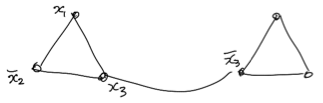
\includegraphics{images/indep_set_traingle.png}
                        \caption{Independent Set from a Triangle}
                        \label{fig:indep_set_traingle}
                    \end{figure}

                    There truth value assignment that satisfies all $k$ clauses iff there is an independent set of $k$ vertices.

                    In particular, $\opt_\text{Max 3-\textsc{sat}}(F) = \opt_\text{Ind. Set} (G)$, and a polynomial time approximation for algorithm for Ind. Set that gives $A_\text{Ind. Set}(G) \ge \alpha \opt_\text{Ind. Set}(G)$ implies a polynomial-time approximation algorithm for the max-\textsc{sat} that gives $A_\text{Max 3-\textsc{sat}}(F) \ge \alpha \opt_\text{Max 3-\textsc{sat}}(F)$.
                % subsection reduction_preserving_constant_factor_approximation (end)
                \subsection{Reduction Preserving Constant Factor Approximation, With a Different Constant} % (fold)
                \label{sub:reduction_preserving_constant_factor_approximation_with_a_different_constant}
                    We give an example where a reduction provides constant-factor approximation, but not the same constant.

                    We allude that the example here is a ``gap-preserving reduction'', but we won't learn more about it in this course.

                    We'd like to show how a polynomial-time $(1 + \varepsilon)$-approximation for Vertex Cover implies a polynomial-time $(1 - 5 \varepsilon)$-approximation for Max 3-\textsc{sat}.

                    From this, we make the observations:
                    \begin{itemize}
                        \item With the breakthrough result from earlier, we now know that there's no \ptas for vertex cover (unless $\p = \np$).
                        \item We have a 2-approximation for Vertex Cover, but this promises us a $(1-5)$-approximation, which is vacuous (and therefor it doesn't apply).
                    \end{itemize}

                    To prove our theorem, we need a reduction Max 3-\textsc{sat} $\le$ vertex cover with a good approximation factor preservation.

                    Using the above, we can reduce Max 3-\textsc{sat} $\le$ Ind. Set, plus the idea that $U$ is an Ind. Set iff $V-U$ is a vertex cover.

                    While this idea doesn't give a good approximation factor in general, but we only need it for graphs that come from Max 3-\textsc{sat}.
                    % TODO: link to 'earlier'
                    From earlier, picking random truth values for Max 3-\textsc{sat}, so $\opt_{\textsc{sat}} \ge \frac{1}{2}m$.

                    $A_\textsc{vc} \le (1 + \varepsilon) \opt_\textsc{vc}$ by assumption.

                    By reduction, we get the approximate polynomial-time for Max 3-\textsc{sat} ``$A_\textsc{sat}$''.
                    \begin{align*}
                        A_\textsc{sat} &= 3m - A_\textsc{vc} \\
                        \opt_\textsc{sat} &= 3m - \opt_\textsc{vc}
                    \end{align*}
                    We want to prove that $A_\textsc{sat} \ge (1 - 5 \varepsilon) \opt_\textsc{sat}$.

                    From the above, we can reduce:
                    \begin{align*}
                        A_\textsc{sat} &= 3m - A_\textsc{vc} \\
                        &\ge 3m - (1 + \varepsilon) \opt_\textsc{vc} \\
                        &= 3m - (1+ \varepsilon)(3m - \opt_\textsc{sat}) \\
                        &= \opt_\textsc{sat} - \varepsilon m + \varepsilon \opt_\textsc{sat} \\
                        &\ge \opt_\textsc{sat} - \varepsilon 6 \opt_\textsc{sat} + \varepsilon \opt_\textsc{sat} \\
                        &= \opt_\textsc{sat} (1 - 5 \varepsilon)
                    \end{align*}

                % subsection reduction_preserving_constant_factor_approximation_with_a_different_constant (end)
            % section polynomial_time_approximation_scheme (end)
        % chapter max_sat (end)
        \chapter{Geometric Packing PTAS} % (fold)
        \label{cha:geometric_packing_ptas}
            We're going to look at packing problems.

            \section{Set Packing} % (fold)
            \label{sec:set_packing}
                We can express set packing through the following statement:
                \begin{quotation}
                    Given elements $\{1, \ldots, n\}$ and sets $\{S_1, \ldots, S_k\}$, with $S_i \subseteq [1, n]$.
                    Find the maximum set of $S_i$ such that no two sets intersect.
                \end{quotation}
                There's a graph version of the same problem:
                \begin{quotation}
                    Given a graph $G = (V, E)$, find a maximum size subset $U \subseteq V$ such that no edge $e = (u, v)$ has both endpoints in $U$.
                \end{quotation}
                The largest Indep. Set (See the definition of this problem inside Section~\ref{sec:vertex_cover}) is a special case of set packing, where all edges incident to vertex $v_i$ is the set $S_i$.

                The independent set problem is \npcomplete, and we can turn general set packing into the independent set problem, therefore set packing is \npcomplete.

                In fact, there is no $n^{1-\varepsilon}$-approximation ratio for independent set, unless $\p = \np$.
            % section set_packing (end)
            \section{Geometric Set Packing With Squares} % (fold)
            \label{sec:geometric_set_packing_with_squares}
                \begin{quotation}
                    Given $n$ unit squares in the plane. Find the maximum number of squares such that no two intersect.
                \end{quotation}
                \subsection{Simple Constant Factor Approximation For Packing Unit Squares} % (fold)
                \label{sub:simple_constant_factor_approximation_for_packing_unit_squares}
                    \begin{lstlisting}
pick_non_intersecting(S[] squares):
    ans = []
    while (|S| != 0):
        sq = s.random()
        s.remove_intersecting(sq)
        ans.append(sq)
    return ans
                    \end{lstlisting}
                    This is a $\frac{1}{4}$-approximation algorithm because at one square chosen by $A$ intersects at most four squares in \opt.

                    Thus, each square of $A$ intersects $\le 4$ squares of \opt.
                    Therefore $\opt \le 4 A$.
                % subsection simple_constant_factor_approximation_for_packing_unit_squares (end)
                \subsection{Grid Approximation Algorithm} % (fold)
                \label{sub:grid_approximation_algorithm}
                    If we represent squares by their center points, and put down a unit grid with the ``even'' squares, we can get the set of points from each of the shaded squares.

                    Let $R_0$ be the set of shaded squares.
                    In fact, we can define:
                    \begin{align*}
                        R_0 &= \{ (x, y) : \myfloor{x} \text{ is even}, \myfloor{y} \text{ is even}\} \\
                        R_1 &= \{ (x, y) : \myfloor{x} \text{ is odd}, \myfloor{y} \text{ is even}\} \\
                        R_2 &= \{ (x, y) : \myfloor{x} \text{ is even}, \myfloor{y} \text{ is odd}\} \\
                        R_3 &= \{ (x, y) : \myfloor{x} \text{ is odd}, \myfloor{y} \text{ is odd}\}
                    \end{align*}
                    The best way to show this is through a figure.
                    Refer to Figure~\ref{fig:grid_approx_alg} for a pictorial example.
                    \begin{figure}[h]
                        \centering
                        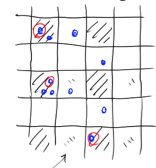
\includegraphics{images/grid_approx_alg.png}
                        \caption{Grid Approximation Algorithm}
                        \label{fig:grid_approx_alg}
                    \end{figure}

                    The algorithm is to take one point from each shaded square $R_0 \cap P$, if there is one.

                    \begin{lstlisting}
grid_approx_alg(P Point[]):
    for i = 0...3:
        Q[i] = opt solution R_i.intersect(P)
    return max(Q)
                    \end{lstlisting}
                    We know that $|Q| \ge \frac{1}{4} \sum |Q_i|$, since we have $\max \ge \text{avg}$.

                    \begin{align*}
                        \opt &= \sum_{i=0}^3 | \opt \cap R_i| \\
                        &\le \sum_{i=0}^3 |Q_i| \\
                        &\le 4|Q|
                    \end{align*}
                    Thus, $|Q| \ge \frac{1}{4} \opt$.
                % subsection grid_approximation_algorithm (end)
                \subsection{Arbitrary Grid Approximation Algorithm} % (fold)
                \label{sub:arbitrary_grid_approximation_algorithm}
                    It turns out that we can get arbitrarily close to an approximation factor of 1, using a ``shifting grid'' approach\footnote{Discovered by Hochbaum \& Maas, `85.}

                    We pick a $k \ge 2$, and let $R_{i, j}$ be defined as:
                    \begin{align*}
                        R_{i, j} &= \{ (x, y): \myfloor{x} \% k \not = i, \myfloor{y} \% k \not = j \}
                    \end{align*}
                    Over $i \in [0, k-1]$ and $j \in [0, k-1]$.
                    Refer to Figure~\ref{} for $k=3$.
                    \begin{figure}[h]
                        \centering
                        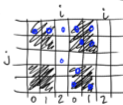
\includegraphics{images/arbitrary_grid_approx_alg.png}
                        \caption{Arbitrary Grid Approximation Algorithm}
                        \label{fig:arbitrary_grid_approx_alg}
                    \end{figure}

                    Note that our points lie in a $n\cdot n$ square without loss of generality.

                    For a given $k$, the number of black squares is $\le \frac{n}{k} \cdot \frac{n}{k} = \frac{n^2}{k^2}$.

                    Also, the number of points we can choose in a single black square is $\le (k - 1)^2$.

                    Since each set of black squares is independent, we can solve the problem optimally for $R_{i,j} \cap P$ in polynomial time by trying all possible subsets of $\le (k-1)^2$ points.
                    There are $O(n^{(k-1)^2})$ possible subsets per square.

                    The algorithm is as follows:
                    \begin{lstlisting}
arbitrary_grid_approximation_algorithm(P, k):
    for i=[0, k-1]:
        for j=[0, k-1]:
            Q[i][j] = R[i][j].intersect(P)
    return max(Q)
                    \end{lstlisting}
                    \begin{align*}
                        \max &\ge \text{avg} \\
                        \implies |Q| \ge \frac{1}{k^2} \sum_{i,j=0}^{k-1} Q_{i, j}
                    \end{align*}
                    Since each point is in $(k-1)^2$ of the $R_{i,j}$'s, then we have:
                    \begin{align*}
                        (k-1)^2 \opt &= \sum_{i,j} | \opt \cap R_{i, j} | \\
                        &\le \sum_{i, j} | Q_{i, j} | \\
                        &\le k^2 | Q |
                    \end{align*}
                    So we have $|Q| \ge \frac{(k-1)^2}{k^2}\opt$ with a runtime $O(k^2 n^{(k-1)^2})$.
                % subsection arbitrary_grid_approximation_algorithm (end)
            % section geometric_set_packing_with_squares (end)
            \section{PTAS-like Definitions} % (fold)
            \label{sec:ptas_like_definitions}
                You'd think that using these for so long, we would've defined this stuff already:
                \begin{description}
                    \item[Approximation Scheme] an algorithm $A$, input $I$ and parameter $\varepsilon$.
                        \begin{itemize}
                            \item For min problem: $A(I, \varepsilon) \le (1 + \varepsilon) \opt(I)$
                            \item For max problem: $A(I, \varepsilon) \ge (1 - \varepsilon) \opt(I)$
                        \end{itemize}
                    \item[Polynomial Time Approximation Scheme (PTAS)] an algorithm $A$ that for each fixed $\varepsilon$, $A$ runs in \p time in $n = |I|$.
                    e.g. $O(n^\frac{1}{\varepsilon})$.
                    \item[Fully Polynomial Time Approximation Scheme (FPTAS)] an algorithm $A$ that runs in \p time in $n = |I|$ and $\frac{1}{\varepsilon}$.
                    e.g. $O(\frac{1}{\varepsilon}^2 n^3)$.
                \end{description}
                For the algorithm described in Subsection~\ref{sub:arbitrary_grid_approximation_algorithm}, the approximation factor $\frac{(k-1)^2}{k^2} = 1 - \frac{2k - 1}{k^2}$, so $\varepsilon = \frac{2k - 1}{k^2}$.

                The runtime is $O(k^2 n^{(k-1)^2})$.
                We have $\varepsilon < \frac{2k}{k} = \frac{2}{k}$, so $k < \frac{2}{\varepsilon}$.
                Also we have $(k-1)^2 < k^2 < \frac{4}{\varepsilon^2}$.
                So we have the overall runtime in $O(\frac{1}{\varepsilon^2} n ^{\frac{4}{\varepsilon^2}})$.
                Thus this is a \ptas but not a \fptas.
            % section ptas_like_definitions (end)
        % chapter geometric_packing_ptas (end)
        \chapter{Bin Packing PTAS} % (fold)
        \label{cha:bin_packing_ptas}
            Bin packing is a cool problem.

            \section{Bin Packing Description and Variants} % (fold)
            \label{sec:bin_packing_description_and_variants}
                \begin{quotation}
                    Given $n$ numbers\footnote{I don't know why she used $S$, given that it usually denotes a set. Oh well.} $S = \{s_1, \ldots, s_n\}$, and $s_i \in [0, 1]$.
                    Pack $S$ into the minimal number of unit bins possible.
                \end{quotation}

                This problem is \nphard, since it generalizes the \textsc{partition} problem:
                \begin{quotation}
                    Given $S$ as above, we can we split $S$ into two bins $U$ and $S-U$ such that:
                    \begin{align*}
                        \sum_{s \in U} s &= \sum_{s \in S-U} s
                    \end{align*}
                \end{quotation}

                There are two variants to this problem:
                \begin{description}
                    \item[Online] numbers in $S$ arrive one at a time and must be inserted to bins immediately.
                    \item[Offline] all numbers in $S$ arrive simultaneously.
                \end{description}
            % section bin_packing_description_and_variants (end)
            \section{First-Fit Bin Packing} % (fold)
            \label{sec:first_fit_bin_packing}
                The first-fit algorithm is really simple:
                \begin{quote}
                    Insert the element into the first bin that fits it.
                \end{quote}
                Due to the algorithm's simplicity, this can be done online.

                Let $m$ be the number of bins used by first fit.
                Since no two bins are $\le \frac{1}{2}$ full, then at least $m - 1$ bins are $> \frac{1}{2}$.
                \begin{align*}
                    \frac{1}{2} (m-1) < \sum s_i \\
                    &\le \opt \\
                    m &< 2\opt + 1
                \end{align*}
                So $m \le 2 \opt$.

                We state without proof that the first fit algorithm uses $\le 1.7 \opt + 1$ bins, and this is tight\footnote{Being tight means that we've proved that it's $\le1.7$, and have infinitely many examples where the algorithm gives this ratio, effectively proving the approximation uses $= 1.7\opt + 1$ bins.}.
            % section first_fit_bin_packing (end)
            \section{First Fit Decreasing Bin Packing} % (fold)
            \label{sec:first_fit_decreasing_bin_packing}
                An off-line algorithm allows us to sort our input in a decreasing order.

                First-fit decreasing sorts $S$ descending, then applies the first fit algorithm.

                We have the asymptotic ration of $\frac{11}{9} = 1.22$, which is tight.
            % section first_fit_decreasing_bin_packing (end)
            \section{PTAS for offline Bin Packing} % (fold)
            \label{sec:ptas_for_offline_bin_packing}
                For any constant $\varepsilon > 0$, there is a polynomial-time algorithm $A'$that uses $\le (1 + \varepsilon)\opt + 1$ bins.

                The ``$+1$ bins'' is crucial:
                \begin{quote}
                    Prove that 2 bins there is no \p time approximation algorithm with an approximation factor of $< 1.5$ (unless $\p = \np$).
                \end{quote}

                The algorithm $A'$ is built from two cases:
                \begin{enumerate}
                    \item $\forall i: s_i \ge \delta$, and there are only $k$ possible values of $s_i$ for constant $k$ and $\delta$.

                        We can solve exactly through brute force enumeration.

                        There are $\le \frac{1}{\delta}$ items in each bin, so there are $k^\frac{1}{\delta}$ ways to fill each bin.
                        Given that there are $\le n$ bins, where each bin has $k^\frac{1}{\delta}$ choices.
                        Overall, we have $O(n^{k^\frac{1}{\delta}})$, which is polynomial for fixed $k$ and $\delta$, but huge.

                        Apparently we can do better with ILP algorithms.
                    \item $\forall i: s_i \ge \delta$ for some constant $\delta$.

                        We convert this to the first case by rounding.

                        Sort values of $s_i$ ascending, and chop every $k$ values of $s_i$ ($k$ is chosen later).

                        Create a set with modified input rounded up to the nearest $s_{\frac{ni}{k}}$:
                        \begin{align*}
                            S^+ &= \{ s_{\frac{n}{k}}, \ldots s_\frac{n}{k}, s_{\frac{2n}{k}}, \ldots s_\frac{2n}{k}, \ldots s_{n}, \ldots s_n \}
                        \end{align*}
                        In other words, there are $\frac{n}{k}$ of $s_{\frac{n}{k}}$.

                        We then apply part 1 to $S^+$.

                        If we define $S^-$ similarly to $S^+$ but instead rounding down instead of up, then we have:
                        \begin{align*}
                            \opt(S^-) &\le \opt(S) \\
                            \opt(S^+) &\le \opt(S^-) + \frac{n}{k} \\
                            &\le \opt(S) + \frac{n}{k}
                        \end{align*}
                        Now $n \delta \le \sum s_i \le \opt(S)$, so $n \le \frac{\opt(S)}{\delta}$.
                        \begin{align*}
                            \opt(S^+) &\le \opt(S) + \frac{\opt(S)}{k\delta} \\
                            &= \opt(S) + \left( 1 + \frac{1}{k \delta} \right)
                        \end{align*}
                        If we set $k = \frac{1}{\delta^2}$, then $\opt(S^+) \le opt(S)(1 + \delta)$.
                \end{enumerate}
                The final algorithm uses case 2 to pack all $s_i$'s where $s_i \ge \delta$, then use first fit to pack the remaining $s_i$'s in the empty spaces of all bins.

                \subsection{Analysis of the PTAS} % (fold)
                \label{sub:analysis_of_the_ptas}
                    Our goal is to prove that $A \le (1 + \varepsilon) \opt + 1$.

                    If the second part does not use new bins, then it's ok to use $\delta = \varepsilon$.

                    Otherwise, we have use $m$ bins in our algorithm.

                    Only the last bin can have size $\le 1 - \delta$, otherwise first fit wouldn't have filled the last bin.
                    Then:
                    \begin{align*}
                        \sum s_i \ge (m-1)(1-\delta) \\
                        m \le \frac{\sum s_i}{1-\delta} + 1 \le \frac{\opt(S)}{1 - \delta} + 1
                    \end{align*}
                    If we choose $\frac{1}{1-\delta} = 1 + \varepsilon$, then we have $\delta = \frac{\varepsilon}{1 + \varepsilon}$ and $m \le (1 + \varepsilon) \opt(S) + 1$ as desired.

                    The runtime is as follows:
                    \begin{align*}
                        O(n^{k^\frac{1}{\delta}}) &= O\left(n^                        {\left( \frac{(1 + \varepsilon)^2}{\varepsilon} \right) ^\frac{1+\varepsilon}{\varepsilon}}
\right)
                    \end{align*}
                % subsection analysis_of_the_ptas (end)
            % section ptas_for_offline_bin_packing (end)
            \section{Improvements for Bin Packing Algorithms} % (fold)
            \label{sec:improvements_for_bin_packing_algorithms}
                Karmarkar and Karp in `82 created an asymptotic $(1 + \varepsilon)$-approximation that runs in $O\left( \left(\frac{1}{\varepsilon} \right)^8 n \log n \right)$ time.
                This is an example of a FPTAS.

                It is \open if we can get $n_\text{bins} \le \opt(S) + O(1)$ in \p time.
            % section improvements_for_bin_packing_algorithms (end)
        % chapter bin_packing_ptas (end)
        \chapter{Knapsack FPTAS} % (fold)
        \label{cha:knapsack_fptas}
            \section{Problem Background} % (fold)
            \label{sec:problem_background}
                \begin{quotation}
                    Give objects $1 \ldots n$, each with size $s_i \in \mathbf{N}$ and profit $p_i \in \mathbf{N}$, given knapsack capacity $B$ find $K \subseteq \{1, \ldots, n \}$ such that $\sum_{i \in K} s_i \le B$ while maximizing $\sum_{i \in K} p_i$.
                \end{quotation}

                The decision version of this problem is \npcomplete\footnote{This can be proved by reducing subset sum to knapsack or partition.}.
            % section problem_background (end)
            \section{Pseudo-Polynomial Time Algorithm for Knapsack with DP} % (fold)
            \label{sec:pseudo_polynomial_time_algorithm_for_knapsack_with_dp}
                We want to find a solution to the knapsack problem using a DP solution.

                A subproblem $S(i, p)$ is defined as the minimum size of the subset of items in $[1, i]$ with profit of exactly $p$.

                Our algorithm is as follows:
                \begin{lstlisting}
knapsack_dp(S[] s, P[] p, B):
    p_max = max(P)
    sums = [n][p_max];
    for p = [1, p_max]:
        if (p == p[1]):
            sums[1][p] = p[1]
        else:
            sums[1][p] = infinity
    for i = [2, n]:
        for p = [1, p_max]:
            sums[i][p] = min(sums[i-1][p], sums[i-1][p-p[i]] + s[i])
    return max p such that sums[n][p] <= B
                \end{lstlisting}

                The runtime of this is $O(n \verb|p_max|)$, which is $O(n^2 \max_i(p_i))$.

                This algorithm is pseudo-polynomial time, since the runtime depends on the largest $p_i$, not on the size of $p_i$'s, which is $\log(p_i)$ bits.

                Some \npcomplete problems don't have pseudo-polynomial time algorithms (unless $\p = \np$).
                For example, \textsc{tsp} is still \npcomplete with $0-1$ weights, since it still can be reduced to the Hamiltonian cycle problem.
            % section pseudo_polynomial_time_algorithm_for_knapsack_with_dp (end)
            \section{FPTAS for the Knapsack Problem} % (fold)
            \label{sec:fptas_for_the_knapsack_problem}
                The idea is that if $p_i$ is few bits, then the pseudo-polynomial time algorithm runs in polynomial time $O(n^2 \max_i (p_i))$.
                So let's round $p_i$'s to have few bits.

                Run the following algorithm for a value of $t$:
                \begin{lstlisting}
knapsack_fptas(epsilon, S[] s, P[] p_initial, B):
    t = ...
    P[] p = new P[p_initial.length]
    for i = [0, p_initial.length]:
        p[i] = floor(p_initial[i]/t)
    return knapsack_dp(s, p, B)
                \end{lstlisting}
                Suppose the result returns $K(t) \subseteq [1, n]$.
                $K(t)$ is feasible, since $\sum_{i \in K(t)} s_i \le B$.

                We need to analyze $P(K(t)) = \sum_{i \in K(t)} p_i$ compared to $P(K^*) = \opt$.

                We know that $p_i - t < tp'_i \le p_i$.
                Then we have:
                \begin{align*}
                    \sum_{i \in K(t)} p_i &\ge \sum_{i \in K(t)} tp'_i \\
                    &\ge \sum_{i \in K^*} tp'_i \\
                    &\ge \sum_{i \in K^*}(p_i - t) \\
                    &= \sum_{i \in K^*}p_i - t|K^*| \\
                    &\ge \opt - t|K^*| \\
                    &\ge \opt - tn \\
                    &= \opt \left(1 - \frac{tn}{\opt}\right) \\
                    &\ge \opt \left( 1 - \frac{tn}{\max_i (p_i)} \right)
                \end{align*}
                We want $\ge \opt(1 - \varepsilon)$, so we choose $t$ such that $\varepsilon = \frac{tn}{\max_i (p_i)}$, and $t = \frac{\varepsilon \max_i p_i}{n}$.

                The runtime is in $O(n^2 \max_i (p'_i))$.
                We know that:
                \begin{align*}
                    p'_i &= \myfloor{\frac{p_i}{t}} \\
                    &= \myfloor{ \frac{n p_i}{\varepsilon \max_i (p_i)}} \\
                    &\le \frac{n}{\varepsilon}
                \end{align*}
                Thus, the runtime is $O(n^3 \frac{1}{\varepsilon})$, which means it's a FPTAS.

                \subsection{Comments on the State-of-the-Art} % (fold)
                \label{sub:comments_on_the_state_of_the_art}
                    The best known algorithm has the runtime $O(n \log \frac{1}{\varepsilon} + \left( \frac{1}{\varepsilon} \right)^4)$.
                    The general idea is to separate it into large profit items and small profit items, then to use the large ones first.
                % subsection comments_on_the_state_of_the_art (end)
                \subsection{FPTAS and Pseudo-Polynomial Time Algorithms} % (fold)
                \label{sub:fptas_and_pseudo_polynomial_time_algorithms}
                    Though we've shown that for the knapsack problem, having a pseudo-polynomial time algorithm $\to$ FPTAS, it's not known (i.e. it's \open) that this is true in general.

                    Garey \& Johnson in `78 proved that if a problem has a FPTAS\footnote{Apparently they made some technical assumptions as well.}, then there must exist a pseudo-polynomial time algorithm for the problem.

                    The idea is that with a minimization problem and a obj function that's integer-valued (this is the technical assumption, I'm not sure what it means), and a bound of $\opt < q (|I_\text{unary}|)$, where $I_\text{unary}$ is the input with numbers expressed in unary and $q$ is some polynomial.

                    Suppose our algorithm $A$ is a FPTAS with runtime $p(|I|, \frac{1}{\varepsilon})$ and $A(I) \le (1 + \varepsilon) \opt(I)$.

                    Picking that $\varepsilon$ small enough to get the \opt, we can argue that this is pseudo-polynomial.
                    \begin{align*}
                        \varepsilon &= \frac{1}{q(|I_\text{unary}|)} \\
                        A(I) &\le (1 + \varepsilon)\opt(I) \\
                        &< \opt(I) + 1
                    \end{align*}
                    Since our obj function is integer valued, we can make the argument that $A$ must give the \opt solution.

                    Thus, the runtime is $p(|I|, \frac{1}{\varepsilon}) = p(|I|, q(|I_\text{unary}|))$, which is pseudo-polynomial time.
                % subsection fptas_and_pseudo_polynomial_time_algorithms (end)
            % section fptas_for_the_knapsack_problem (end)
        % chapter knapsack_fptas (end)
        \chapter{Hardness of Approximation} % (fold)
        \label{cha:hardness_of_approximation}
            In general, some \npcomplete problems can be approximated in different manners.

            Listed from hardest to easiest, we have:
            \begin{itemize}
                \item $O(n^\varepsilon)$ - factor
                \item $O(n \log n)$ - factor (Set Cover)
                \item Constant factor (Vertex Cover, Euclidean TSP)
                \item \ptas (Packing Unit Squares, Bin Packing)
                \item \fptas (knapsack)
            \end{itemize}

            If the positive results give an approximation algorithm, then negative results give that it's hardest.

            We can show that a \ptas for vertex cover existing implies that $\p = \np$.

            For the Max-3SAT problem, we know through reductions that a \ptas for either vertex cover or Independent Set implies that there must be a \ptas for Max-3SAT, since there are reductions preserving good approximations.

            \section{A New Definition of \np} % (fold)
            \label{sec:a_new_definition_of_np}
                Earlier, we defined \np as a set of decision problems verifiable in \p given a certificate of polynomial size.

                If we think about this as a game between the prover $P$ (who finds the certificate) and the verifier $V$ (verifies the problem), then we can get some edge by talking about how much $V$ asks $P$ and how much $V$ guesses randomly.

                An interactive proof system is essentially what we're building. $V$ asks $P$ about parts of the proof, and guesses\footnote{$P$ does not infer, but guesses randomly.} some others.
                \subsection{Graph Isomorphism} % (fold)
                \label{sub:graph_isomorphism}
                    \begin{quotation}
                        Given 2 graphs $G_1$ and $G_2$, can you relabel $G_1$ to get $G_2$?
                    \end{quotation}
                    Graph isomorphism is in \np, but it is \open if it is in \p or in \npcomplete.

                    For the $V$, we can pick one of $G_1$ or $G_2$ at random, and ask $P$ about which one we relabeled.

                    \begin{itemize}
                        \item If $G_1 \not= G_2$, then the prover can answer correctly.
                        \item If $G_1 = G_2$, then the prover can't do better than 50\% right.
                    \end{itemize}
                    Thus $V$ runs many trials to verify $G_1 \not= G_2$ with high probability.

                    This is a restricted instance, since there are no rounds and only one prover\footnote{Apparently there are instances where more than one prover is necessary, but I can't think of any.}.
                % subsection graph_isomorphism (end)
                \subsection{Probabilistically Checkable Proofs} % (fold)
                \label{sub:probabilistically_checkable_proofs}
                    Given a result to a decision problem, we have a game between the Prover and Verifier.
                    \begin{itemize}
                        \item Prover writes the ``proof''.
                        \item The Verifier is a randomized algorithm that ``checks'' the proof and answers \textsc{yes} or \textsc{no}.
                    \end{itemize}
                    If the statement is true, then there is (always?) a proof that makes $V$ (always?) answer \textsc{yes}.

                    If the statement is false, then $V$ must answer \textsc{no} with $\text{Pr} \ge \frac{3}{4}$, no matter the proof given.

                    If we limit $V$ to $O(f(n))$ random bits, and $O(g(n))$, then we define \textsc{pcp} as follows:

                    \begin{quote}
                        $\textsc{pcp}[f, g]$ is the class of decision problems with Probabilistically Checkable Proof where $V$ uses $O(f(n))$ random bits, and $O(g(n))$ bits of the proof.
                    \end{quote}
                    We have $\textsc{pcp}[0, \text{poly}(n)] = \np$, and $\textsc{pcp}[0, 0] = \p$.
                % subsection probabilistically_checkable_proofs (end)
                \subsection{PCP Theorem} % (fold)
                \label{sub:pcp_theorem}
                    The ``PCP Theorem'' is by (Aurora, Lund, Motwani, Sudan, and Szegedy in `92).
                    It states that:
                    \begin{align*}
                        \np &= \textsc{pcp}[\log n, 1].
                    \end{align*}
                    Essentially, $V$ uses \uline{random bits} to choose \uline{where} to look at the proof.

                    Proving $\textsc{pcp}[\log n, 1] \subseteq \np = \textsc{pcp}[0, \text{poly}(n)]$ is not hard, since the verifier only needs to eliminate randomness and tries all possible random strings of $O(\log n)$ bits.
                    It then looks at $n^k$ bits of the proof.

                    The other direction is hard.
                % subsection pcp_theorem (end)
                \subsection{Implications of the PCP Theorem to Hardness of Approximation} % (fold)
                \label{sub:implications_of_the_pcp_theorem_to_hardness_of_approximation}
                    From the \textsc{pcp} theorem, we know that a \ptas for Max 3-SAT implies that $\p = \np$.

                    Using $\np = \textsc{pcp}[\log n, 1]$, we can take any problem in $\np$ and the $\textsc{pcp}[\log n, 1]$ verifier's algorithm for it.

                    The algorithm depends on the input bits $x_1, \ldots, x_n$, the proof bits $y_1, \ldots, y_t$ (for $t \in O(\text{poly}(n))$), and the random bits $r_1, \ldots, r_k$ (for $k \in O(\log n)$).

                    We can reduce any\footnote{Maybe any  \npcomplete?} algorithm to a Boolean 3-SAT formula.

                    Using variables for $y_1, \ldots, y_t$, we can choose the formula $F(x, y, r)$ to capture the verifier's algorithm.

                    Let $F(x, y) = \land_{r} F(x, y, r)$.

                    Since $r$ is polynomial size, we can say the following:
                    \begin{itemize}
                        \item if $x$ is \textsc{yes} input, then there exists a $y$ such that all $F(x, y, x)$ are satisfied and thus $F(x, y)$ is satisfied.
                        \item if $x$ is \textsc{no} input, then for any $y$, at most $\frac{1}{4}$ of the $F(x, y, x)$ are satisfied, and at most a fraction of the clauses of $F(x, y)$ can be satisfied.
                    \end{itemize}
                    By having a gap when $x$ is a \textsc{no} input between \opt and ``all'', we can detect this gap with a good approximation algorithm.
                % subsection implications_of_the_pcp_theorem_to_hardness_of_approximation (end)
            % section a_new_definition_of_np (end)
        % chapter hardness_of_approximation (end)
        \chapter{Online Algorithms} % (fold)
        \label{cha:online_algorithms}
            Given a sequence of requests, our algorithm must handle each request as it comes.
            This is the usual scenario for data structures, but we will study situations where it makes sense to compare with complete solutions.

            \begin{itemize}
                \item Bin packing: (first vs best fit)
                \item Splay Trees - dynamic optimality conjecture
                \item Paging (LRU and LFU)
                \item Ski rental - rental is \$30, but purchasing skiis is \$300.
            \end{itemize}

            \section{Robots Finding Doors} % (fold)
            \label{sec:robots_finding_doors}
                Suppose we have a robot an unknown distance $d$ away from a door in an unknown direction.

                In an \opt route, we can provide a solution in length $d$.

                \subsection{Algorithm 0} % (fold)
                \label{sub:algorithm_0}
                    \begin{verbatim}
find_door_0():
    i = 0
    while (true):
        i++
        go i steps right
        go 2i steps left
        go i steps right
        if seen_door():
            goto door
                    \end{verbatim}
                    This takes $4(\sum_i^{d-1}) + d$ steps if the door is on the right, and $4(\sum_i^{d-1}) + 3d$ steps if the door is on the left, so this runs in $\theta(d^2)$ time.
                % subsection algorithm_0 (end)
                \subsection{Algorithm 1} % (fold)
                \label{sub:algorithm_1}
                    \begin{verbatim}
find_door_1():
    i=0
    while (true):
        i++
        if i is odd:
            go 2^i steps right
            go 2^i steps left
        else: // (i is even)
            go 2^i steps left
            go 2^i steps right
                    \end{verbatim}
                    If $2^i \le d \le 2^{i+1}$, then the distance travelled is $\le 2\sum_j^{i+1} j^2 + d$.
                    Thus the distance travelled $\le 2 (2^{i+2} - 1) + d \le 2 (4d + 1) + d \le 9d$.

                    Since we know the distance travelled is $9d$, then we have what we call a competitive ratio of $9$.
                % subsection algorithm_1 (end)
                \subsection{Algorithm 2} % (fold)
                \label{sub:algorithm_2}
                    This is a randomized version of the algorithm.

                    Flip a coin to choose th initial direction - $f \in \{0, 1\}$.

                    Then we do the algorithm described in Section~\ref{sub:algorithm_1}.
                    The odd/even test becomes $i \mod 2 = f$, and we now get to see the expected distance travelled:
                    \begin{align*}
                        2(\sum_j 2^j) + \frac{1}{2} 2(2^{i+1}) + d \\
                        &= 2(2^{i+1} - 1) + 2(2^{i+1}) + d \\
                        &\le 2(2d - 1) + 2d + d \\
                        &\le 7d
                    \end{align*}
                    We have a competitive ratio of $7$ in this case.
                % subsection algorithm_2 (end)
                \subsection{Algorithm 3} % (fold)
                \label{sub:algorithm_3}
                    The best randomized algorithm has a competitive ratio of $4.592$.
                    Let's take a look at it.

                    For a value of $r$ chosen below, do the following algorithm:
                    \begin{verbatim}
find_door_3():
    f = random_bit()
    x = random_float(0, 1)
    i = 0
    while (true):
        if i %2 = f:
            walk r^{i+x} right
            walk r^{i-x} left
        else:
            walk r^{i+x} left
            walk r^{i-x} right
        ++i
                    \end{verbatim}
                    It can be shown that the expected distance travelled $\le \frac{r+1}{\ln r} + 1$, which is minimized when $r = 3.59$, giving the distance $4.59d$.

                    This is the best known approximation factor.
                % subsection algorithm_3 (end)
                \subsection{Further Expansion} % (fold)
                \label{sub:further_expansion}
                    This becomes harder in 2D, as a robot is trying to find an unknown shape in a plane.
                % subsection further_expansion (end)
            % section robots_finding_doors (end)
            \section{Auction Strategies} % (fold)
            \label{sec:auction_strategies}
                There is an item of value $B$, and the auction bids occur one at a time.
                These bids are more like offers, since the algorithm must accept or reject bids immediately as they arrive.
                All bids are positive nonzero integers.

                We want $A(\sigma) \ge c \opt(\sigma) + b$, where $c \le 1$.

                If the number of bids is unknown, then the algorithm must accept the first bid, or else $\frac{A}{\opt} = 0$.

                Supposing the number of bids is known, the algorithm accepts the first bid above some threshold $T$, otherwise it accepts the last bid.

                Supposing the maximum bid is $M \le B$, then $\opt = M$.

                If $T = 2$ and $M \ge 2$, $\frac{2}{M} \ge \frac{2}{B}$.
                If $T = 1$ and $M = 1$, then $\frac{1}{1} = 1$.
                It's best to have the highest $T$ possible.

                \subsection{Deterministic $T$ Threshold} % (fold)
                \label{sub:t_threshold}
                    If we set $T = \myfloor{\sqrt{B}}$, we claim that the competitive ratio is $\frac{1}{\sqrt{B}}$.

                    If $M> \myfloor{\sqrt{B}}$, then in the worst case $A$ accepts $\myfloor{\sqrt{B}} + 1$.
                    The competitive ratio is $\frac{\myfloor{\sqrt{B}} + 1}{M} \ge \frac{\myfloor{\sqrt{B}} + 1}{B} \ge \frac{1}{\sqrt{B}}$.

                    If $M \le \myfloor{\sqrt{B}}$, then the algorithm accepts the last bid.
                    In the worst case, that bid is $1$, so the competive ratio is $\frac{1}{\sqrt{B}}$.

                    In either case, the competitive ratio is $\frac{1}{\sqrt{B}}$.
                % subsection t_threshold (end)
                \subsection{Random $T$ Threshold} % (fold)
                \label{sub:random_threshold}
                    Choose a random $i$ threshold from $i \in [i, \log B]$, then set $T = 2^i$.

                    The worst case is that no bid is occurs $\ge 2^i$, so $A$ gets $0$.

                    We want to prove the expected competitive ratio is $\ge O\left( \frac{1}{\log b} \right)$.

                    Suppose that $M$ is the max bid, so $\opt = M$.

                    Suppose that $2^k \le M < 2^{k+1}$.
                    The probability that we choose $i=k$ is $\frac{1}{\log B}$.

                    For $i = k$, $A$ gets $\ge 2^k \ge \frac{M}{2}$.

                    Thus the expected value for the algorithm is $\ge \frac{M}{2 \log B}$.
                    Then, $\frac{A}{\opt} \ge \frac{1}{2 \log B}$.
                % subsection random_threshold (end)
            % section auction_strategies (end)
        % chapter online_algorithms (end)
        \chapter{Paging} % (fold)
        \label{cha:paging}
            An online algorithm is $c$-competitive if there exists a constant $b$ such that $A(\sigma) \le c\opt(\sigma) + b$.

            We define the paging problem as follows:
            \begin{quote}
                We are given a ``cache'' of fast memory that holds $k$ elements, and a ``disk'' of slow memory that holds $n >> k$ pages.

                When a page is requested, if it's in the cache, we have no problem.

                Otherwise, we ``page fault'' and read the page into the cache at a cost of 1, evicting at least one page to do it.

                We'd like to choose a page eviction strategy with a minimal cost.
            \end{quote}
            \section{Optimum Offline Strategy} % (fold)
            \label{sec:optimum_offline_strategy}
                The optimum strategy is to evict the page with the next request furthest in the future.
                The proof is done from the observation that we can modify any optimum solution to this one, decision by decision.
            % section optimum_offline_strategy (end)
            \section{Online Cache Strategies} % (fold)
            \label{sec:online_cache_strategies}
                \begin{description}
                    \item[FIFO] - first in first out
                    \item[LRU] - least recently used
                    \item[LFU] - least frequently used
                \end{description}
                \subsection{LRU vs FIFO} % (fold)
                \label{sub:lru_vs_fifo}
                    Despite LRU being better than FIFO in practice, both LRU and FIFO have competitive ratio $k$.

                    We can prove this by dividing a request sequence into phases.
                    A phase stops just before the $k+1$th different page is requested.

                    The algorithms use $\le k$ swaps per page, since LRU and FIFO will not evict a page used in that single phase.
                    We know that \opt must evict $\ge 1$ page per phase, because there are $k+1$ distinct pages involved.
                    Thus, we have $\frac{A}{\opt} \le k$, plus an additive constant for a partial phase at an end of a request sequence.
                % subsection lru_vs_fifo (end)
                \subsection{Limitations of Deterministic Selection} % (fold)
                \label{sub:limitations_of_deterministic_selection}
                    We'd like to prove that any deterministic algorithm has competitive ratio $\ge k$.

                    If $k$ is the cache size, and the number of pages is $k+1$, and the adversary can always supply a sequence of length $n$ asking for the page known not to be in the cache.

                    Since there are $n$ swaps in a sequence of length $n$, and we know that a perfect solution subjected to this adversary would use $\frac{n}{k}$ swaps, because each time it evicts, it must be good for the next $k$ requests.

                    Then we have $\frac{A}{\opt} \ge k$ for all deterministic algorithms.
                % subsection limitations_of_deterministic_selection (end)
                \subsection{Randomized Page Swapping Algorithm} % (fold)
                \label{sub:randomized_page_swapping_algorithm}
                    This randomized algorithm is attributed to Fiat in `91.
                    \begin{verbatim}
serve(p):
    p.makeRecent()
    if !cache.contains(p):
        if all pages are recent
            pages.all.makeNotRecent()
        evict a random non-recent page
                    \end{verbatim}
                    Without proof, the expected competitive ratio is $\Theta(\log k)$, which is the best possible for randomized algorithms, assuming the adversary does not see the random choices.
                % subsection randomized_page_swapping_algorithm (end)
            % section online_cache_strategies (end)
            \section{$k$-Server Problem} % (fold)
            \label{sec:k_server_problem}
                The problem formulation is as follows:
                \begin{quote}
                    There are $k$ servers to service requests in metric space at points $\{p_1, \ldots, p_n\}$.

                    When a request for $p_i$ occurs, if a server is at $p_i$, fine.

                    Otherwise, move a server from its location ($p_j$) to $p_i$ at cost $d(p_j, p_i)$.

                    We'd like to serve requests in a given order while minimizing the total distance.
                \end{quote}
                Paging is a special case of this algorithm where $d(p_i, p_j) = 1$ for all $i$, $j$.

                Without proof, we state that the offline algorithm can solve the problem in poly-time.

                \subsection{Greedy Online Algorithm} % (fold)
                \label{sub:greedy_online_algorithm}
                    Given that all points are in 2D, our heuristic is to move the closest server to the point.

                    This unboundedly bad, as a sequence of $(p_1, p_2, p_1, p_2, \ldots)$ will take more time than necessary.

                    It is \open\footnote{Since 1988, the time is apparently nigh} if there is a $k$-competitive algorithm that solves the problem, in any dimension.

                    The best known algorithm is $(2k-1)$-competitive (`94).
                % subsection greedy_online_algorithm (end)
                \subsection{$k$-Competitive Algorithm for Points on a Line} % (fold)
                \label{sub:k_competitive_algorithm_for_points_on_a_line}
                    For points on a line, we split up requests $r_i$ into three types:
                    \begin{enumerate}
                        \item If $r_i$ is to the right of all servers, move the rightmost server right.
                        \item If $r_i$ is to the left of all servers, move the leftmost server left.
                        \item If $r_i$ is between two servers $s_a$, $s_b$, move them both towards $r_i$, stopping both when one reaches the request.
                    \end{enumerate}
                    If multiple servers arrive at the same location, break ties arbitrarily.

                    We present that (without proof) this algorithm is $k$-competitive.
                % subsection k_competitive_algorithm_for_points_on_a_line (end)
            % section k_server_problem (end)
        % chapter paging (end)
        \chapter{Fixed Parameter Tractable Algorithms I} % (fold)
        \label{cha:fixed_parameter_tractable_algorithms_i}
            We know that \npcomplete problems seem to only have exponential time algorithms, but we'd like to classify ``how exponential'' these problems are.

            \section{Completing Problems with Fixed Parameters} % (fold)
            \label{sec:completing_problems_with_fixed_parameters}
                When solving the Vertex Cover problem to find $C \subseteq V$ such that every edge has at least one end point in $C$.

                Say that $k$ is the minimum size vertex cover, and $k$ is known.

                We try to find all subsets of $k$ vertices ${n \choose k} O(n^k) = O({n \choose k} n^k) = O(k n^{k+1})$, which is polynomial time for constant $k$.

                The same idea works for both clique and independent set but not for graph coloring\footnote{Given a graph, is it 3-colorable is \npcomplete, so we still run into that issue.}.

            % section completing_problems_with_fixed_parameters (end)
            \section{A feel for Fixed Parameter Tractable Algorithms} % (fold)
            \label{sec:a_feel_for_fixed_parameter_tractable_algorithms}
                While $O(n^k)$ is not exponential, it's still pretty bad.

                We'd much prefer $O(f(k) n^c)$ for some polynomial $f(k)$ independent of $n$ and some constant $c$ independent of $k$.
                Even better would be $O(f(k) + n^c)$.

                \subsection{FPTA for Vertex Cover} % (fold)
                \label{sub:fpta_for_vertex_cover}
                    We want to build a FPTA for Vertex Cover by branching on all possibilities that for $e = (u, v)$, either $u$ or $v$ is in $C$ (where $C$ is the cover).

                    At each tree, we pick an uncovered edge to branch on.

                    \begin{lstlisting}
vertex_cover(E, V, k):
    if E == {} return true
    if k == 0 return false
    pick e = E.random()
    (u, v) = e
    return vertex_cover(E.without_incident(u), V-u, k-1)
        || vertex_cover(E.without_incident(v), V-v, k-1)
                    \end{lstlisting}
                    The tree has depth $k$, so we take time $O(2^k n)$.

                    By modifying the algorithm, we can trivially find the vertex cover itself.
                % subsection fpta_for_vertex_cover (end)
                \subsection{Kernelization} % (fold)
                \label{sub:kernelization}
                    If we wanted to, we can improve the Vertex Cover technique to $O(f(k) + n^c)$ using kernelization.

                    Essentially, if there exists a vertex $v$ with $\text{deg}(v) > k$, then $v$ must be in the cover $C$, otherwise we'd need all neighbors of $v$ (of which there are $>k$) to be in $C$.
                    \begin{lstlisting}
vertex_cover_kernelized(E, V, k):
    c_2 = all vertexes with deg(v) > k
    k_2 = k - |C_2|
    V_2 = V - C_2
    E_2 = E.without_any_incident(C_2).remove_isolated()
    if |V_2| > 2k^2
        return false
    return VC(E_2, V_2, k_2)
                    \end{lstlisting}
                    The actual vertex cover is $C' \cup \textsc{VC}(E', V', k')$
                    We know that the maximum degree in $V'$ is $\le k$.
                    If $(V', E')$ has a vertex cover of size $\le k$, then $V'$ has $\le k^2$ edges.
                    So $|E'| \le 2k^2$, which is not very big.

                    The idea of kernalization is due to Prof. J. Buss in `93.

                    The call to \textsc{vc} takes $O(2^k |E'|) = O(2^k 2 k^2)$, and finding $C'$ takes $O(m + n)$ time.
                    Thus, the total run time is $O(2^k k^2 + m + n)$.
                % subsection kernelization (end)
            % section a_feel_for_fixed_parameter_tractable_algorithms (end)
            \section{Defining Fixed Parameter Tractable Algorithms} % (fold)
            \label{sec:defining_fixed_parameter_tractable_algorithms}
                A problem is \uline{fixed parameter tractable} (FPT) in parameter $k$ if it has an algorithm\footnote{The algorithm is a Fixed-Parameter Tractable Algorithm (FPTA).} with runtime $O(f(k) n^c)$, wher $n$ is the input size, $f(k)$ is independent of $n$, and $c$ is a constant independent of $k$.

                Given a FPT problem, we can get an algorithm with runtime $O(f'(k) + n^{c'})$.
                This is neither deep, indicative on how to construct this, nor useful, but is interesting.

                \subsection{Common Parameter Examples} % (fold)
                \label{sub:common_parameter_examples}
                    We can pick a few types of examples of parameters:
                    \begin{itemize}
                        \item Value of the \opt solution
                        \item Maximum degree of the graph
                        \item Dimension for geometric problems
                        \item Genus of a graph\footnote{Apparently, this means 0 for planar graphs, and 1 for embeddable on a torus without crossing edges.}
                    \end{itemize}
                    % TODO: make this a link.
                    Refer to Chapter 23 for many FPTA examples.
                % subsection common_parameter_examples (end)
            % section defining_fixed_parameter_tractable_algorithms (end)
            \section{Randomized FPT Algorithm for $k$-Path} % (fold)
            \label{sec:randomized_fpt_algorithm_for_k_path}
                \begin{quotation}
                    Given graph $G$, $k \in \mathbf{N}$, and a starting vertex $s$ and an end vertex $t$, find a simple\footnote{Don't repeat vertexes.} $s \to t$ path with $k$ internal vertexes.
                \end{quotation}
                In general, this is a \nphard problem, since if $k = n-2$, we're asking for a Hamiltonian Path $s \to t$.

                With the power of randomness, we can save the day!

                Randomly color all vertexes into $k$ different colors.
                Then look only for paths that use all $k$ colors.

                The algorithm will always say ``\textsc{no}'' correctly, since it will never find a simple $k$-path within the coloring.

                If there does exist a simple path $P$, we can say the following:
                \begin{align*}
                    \text{Pr}(\text{P is colorful}) &= \frac{k!}{k^k} \\
                    &\ge \frac{\left( \frac{k}{e} \right)^k}{k^k} \\
                    &= \frac{1}{e^k}
                \end{align*}
                So the algorithm is correct when it says ``\textsc{yes}'' with a probability $\ge \frac{1}{e^k}$.

                Defining $p = \frac{1}{e^k}$, then we can say:

                Since $A$ is correct with Probability $\ge p$, then after $\frac{1}{p}$ repetitions, the probability of failure is
                \begin{align*}
                    (1 - p)^{\frac{1}{p}} &< (e^{-p}) ^ \frac{1}{p} \\
                    &= \frac{1}{e}
                \end{align*}
                In our case, repeating $e^k$ times gives us the probability of error $\le \frac{1}{e}$.

                Finding a colorful path for a given ordering is easy, so we find all of them.

                The runtime of setting up and searching orderings is $O(k! m)$, so the final runtime is $O(e^k 2^k m)$, with a probability of error of $\le \frac{1}{e}$.
            % section randomized_fpt_algorithm_for_k_path (end)
        % chapter fixed_parameter_tractable_algorithms_i (end)
        \chapter{Fixed Parameter Tractable Algorithms II} % (fold)
        \label{cha:fixed_parameter_tractable_algorithms_ii}
            The Independent set problem is expressed as follows:
            \begin{quotation}
                Given a graph $G$, does it have an independent set\footnote{of vertexes that share no edges} $\ge k$?
            \end{quotation}
            The brute-force time is $O(n^k (n+m))$, where there are $k$ subsets of $n$ vertexes.
            The brute-force solution \uline{not} FPT.

            In fact, it is \open if there is a FPTA for Independent Set (and this parameter), and it's also \open if existence of a FPTA implies $\p = \np$.

            \section{FPTA for Independent Set} % (fold)
            \label{sec:fpta_for_independent_set}
                The general idea is to use a parameter for a FPTA that measures the ``tree-ness'' of our graph.

                \subsection{Independent Set on a Tree} % (fold)
                \label{sub:independent_set_on_a_tree}
                    We want to find the independent set on a tree.

                    We define the recursive functions $IS(v)$ and $IS'(V)$, which are the maximum weight of the independent set of the subtree rooted at $v$ that do ($IS(v)$) or do not ($IS'(v)$) include $v$.

                    We can even put weights on vertexes as $w(v)$.

                    \begin{lstlisting}
ind_set_tree(V):
    for v = V.leaves:
        IS_2[v] = 0
        IS[v] = w(v)
    for v in V.vertexes-in-leaf-to-root-order:
        // where v_i are the children of v...
        IS_2[v] = sum_i(IS[v_i])
        IS[v]  = max(w(v) + sum_i(IS_2[v_i]), IS_2[v])
    return IS[root]
                    \end{lstlisting}
                % subsection independent_set_on_a_tree (end)
                \subsection{Independent Set on Graphs that are ``Almost'' Trees} % (fold)
                \label{sub:independent_set_on_graphs_that_are_almost_trees}
                    \subsubsection{Series Parallel Graphs} % (fold)
                    \label{ssub:series_parallel_graphs}
                        A Series-Parallel graph (SP) is defined recursively as:
                        \begin{itemize}
                            \item A single edge connecting two vertexes.
                            \item Two parallel SP graphs sharing the same start and end vertexes.
                            \item Two SP graphs connected in series.
                        \end{itemize}
                        Refer to Figure~\ref{fig:sp_composition} for an example.
                        \begin{figure}[h]
                            \centering
                            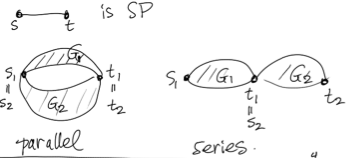
\includegraphics{images/sp_composition.png}
                            \caption{Composition of SP Graphs}
                            \label{fig:sp_composition}
                        \end{figure}
                        We can find the Independent set in series parallel graph by dynamic programming based on the maximum independent set for all permutations containing or not containing $s$ or $t$.
                    % subsubsection series_parallel_graphs (end)
                    \subsection{Decomposing Series Parallel Graphs} % (fold)
                    \label{sub:decomposing_series_parallel_graphs}
                        We can model the decomposition of a SP as a tree.

                        Vertexes that represent a parallel decomposition are a 2-tuple of $(s, t)$.
                        Vertexes that represent a series decomposition are a 3-tuple of $(s, v_\text{middle}, t)$.
                        Edges in the graph appear as leaf vertexes.

                        We have two properties:
                        \begin{enumerate}
                            \item If $e = (u, v)$ is an edge of $G$ then $u$ and $v$ trivially appear together in a tree node.
                            \item Every vertex $v$ of $G$ corresponds to a sub-tree $T$.
                        \end{enumerate}
                    % subsection decomposing_series_parallel_graphs (end)
                    \subsection{Generalization to General Graphs} % (fold)
                    \label{sub:generalization_to_general_graphs}
                        The concept of Tree-Width was created by Robertson \& Seymour as part of the ``Graph Minors Project'', the result of 20 papers, totaling around 500 pages.

                        We want to represent a graph as a tree, and have properties 1 and 2 from above.

                        I believe that we define bags as a 2-or-3-tuple of a vertex.

                        The width of a decomposition is the size of the largest bag in the tree - 1.

                        The tree width of $G$ is the minimum width of any tree decomposition, which is $\le n - 1$.

                        And we only need $\le n$ bags in any tree decomposition.

                        Finding the tree-width of a graph is \nphard, but there is a FPT algorithm $O(2^{O(k^3} n)$.
                    % subsection generalization_to_general_graphs (end)
                % subsection independent_set_on_graphs_that_are_almost_trees (end)
                \subsection{Graphs of Tree Width} % (fold)
                \label{sub:graphs_of_tree_width}
                    The maximum weight of the independent set in a graph of a tree-width $k$ can be found in time $O(2^k n)$.

                    The idea of the proof is to use DP to the tree upwards.

                    For each bag $B$ of size $\le k + 1$ we find for each subset $A \subseteq B$ (there are $O(2^k)$ of them), a maximum weight independent set including $A$ (excluding $B - a$) in the subtree rooted at $B$.
                % subsection graphs_of_tree_width (end)
                \subsection{Other Problems FPT in Tree-Width} % (fold)
                \label{sub:other_problems_fpt_in_tree_width}
                    \begin{itemize}
                        \item 3-Coloring
                        \item Minimum coloring
                        \item Hamiltonian cycle (apparently it's even more complicated)
                    \end{itemize}
                % subsection other_problems_fpt_in_tree_width (end)
                \subsection{Hardness Results of FPT Problems} % (fold)
                \label{sub:hardness_results_of_fpt_problems}
                    All relative results are of the form:
                    A FPT algorithm existing for $X$ implies there is a FPT algorithm for $Y$, and is proved through a reduction that preserves the parameter and the FPT.
                % subsection hardness_results_of_fpt_problems (end)
            % section fpta_for_independent_set (end)
        % chapter fixed_parameter_tractable_algorithms_ii (end)
    % part approximating_ _hard_ _things_ (end)
\newpage
\appendix
    \chapter{Sample Algorithms} % (fold)
    \label{cha:sample_algorithms}
        \section{QuickSort} % (fold)
        \label{sec:quicksort}
            We have data $S = \{ s_1 \ldots s_n \}$.
            \begin{lstlisting}
def QuickSort(S):
    if n == 0 or n == 1:
        return S
    i = random(1, n)
    L = {s_j : s_j < s_i}
    M = {s_j : s_j = s_i}
    R = {s_j : s_j > s_i}
    return QuickSort(L).append(M).append(QuickSort(R))
            \end{lstlisting}
            In the worst case, this runs in $T(n) = T(n-1) + O(n) = O(n^2)$ time.

            We ``expect'' the pivot to be in the middle, so $|L| = |B| = \frac{n}{2}$ and $T(n) = 2 T(\frac{n}{2}) + O(n) = O(n \log n)$.\footnote{In this case, we use ``expectations'' that the input is ``average'', which is not amortized analysis. Better analysis is below.}

            More formally, we'll analyze randomized QuickSort with recursive calls of $T(\ell) + T(n - \ell - 1)$.

            By random choice of pivot, $\ell$ is equally likely to be each of $\{0 \ldots n-1\}$, each with a $\Pr(\frac{1}{n})$.
            Then, we get:
            \begin{align*}
                T(n) &= \frac{1}{n} \left(\sum^{n-1}_{\ell = 0} T(\ell) + T(n - \ell - 1)\right) + O(n) \\
                &= \frac{2}{n} \left(\sum^{n-1}_{\ell = 0} T(\ell)\right) + O(n)
            \end{align*}
            Using a proof by induction, we arrive at $T(n) = O(n \log n)$, which means that we can expect quicksort to take $O(n \log n)$ time\footnote{In CLRS, there is nice analysis without recurrence relations.}.
        % section quicksort (end)
    % chapter sample_algorithms (end)

    \chapter{Math Review} % (fold)
    \label{cha:math_review}
        \section{Expected Values - Statistics} % (fold)
        \label{sec:expected_values_statistics}
            The expected value of the random variable $X$ is $E(X)$.
            For discrete $X$, we know:
            \begin{align*}
                E(X) &= \sum_x xPr\{X = x\}
            \end{align*}
            For any $X$ and $Y$, we know that:
            \begin{align*}
                E(X + Y) &= E(X) + E(Y)
            \end{align*}
            For a constant $c$, we know:
            \begin{align*}
                E(cX) &= cE(X)
            \end{align*}
            If $X$ and $Y$ are independent random variables, we know:
            \begin{align*}
                Pr\{X = x \text{ and } Y = y\} &= Pr\{X = x\} Pr\{Y = y\} \\
                E(XY) &= E(X) E(Y)
            \end{align*}
            More details are in CLRS.
        % section expected_values_statistics (end)
        \section{Markov's Inequality} % (fold)
        \label{sec:markov_s_inequality}
            If the random variable $X \ge 0$ and $E(X) = \mu$, then $\Pr\{ X \ge c \mu \} \le \frac{1}{c}$ for a constant $c$.

            \begin{align*}
                \mu &= E(X) \\
                &= \sum x \Pr(X = x) \\
                &\ge \sum_{x \ge c \mu} x \Pr(X = x) \\
                &\ge c \mu \sum_{x \ge c \mu} \Pr(X = x) \\
                &= \Pr(X \ge c \mu) \\
                \Pr(X \ge c \mu) &\le \frac{\mu}{c \mu} \\
                &= \frac{1}{c}
            \end{align*}
            This proof can be found on page 5 of the Lecture 11 notes.
        % section markov_s_inequality (end)
        \section{Logic} % (fold)
        \label{sec:logic}
            \subsection{Contrapositive} % (fold)
            \label{sub:contrapositive}
                The contrapositive is defined as $(A \implies B) \implies (\lnot B \implies \lnot A)$.
            % subsection contrapositive (end)
            \subsection{Conjunctive Normal Form (CNF)} % (fold)
            \label{sub:conjunctive_normal_form_}
                Given a boolean formula, \textsc{CNF} is the form:
                \begin{align*}
                    E &= (x_1 \lor x_2 \lor x_3) \land (x_1 \lor \lnot x_2) \land (\lnot x_1 \lor \lnot x_2 \lor \lnot x_3) \land (x_2 \lor \lnot x_3)
                \end{align*}
            % subsection conjunctive_normal_form_ (end)
        % section logic (end)
    % chapter math_review (end)
\end{document}

% Covered so far: Lecture 13 notes.
